\documentclass[12pt]{article}

% фонтови и језик
% fontspec docs: shorturl.at/ouI26
\usepackage{fontspec}

% polyglossia docs: shorturl.at/gELX9
\usepackage{polyglossia}
\newfontfamily\cyrillicfont{Times New Roman} % може се заменити компатибилним фонтом
\newfontfamily\cyrillicfontsf{Arial}         % може се заменити компатибилним фонтом
\newfontfamily\cyrillicfonttt{Courier New}   % може се заменити компатибилним фонтом
\setmainlanguage[Script=cyrillic]{serbian}
\setotherlanguage{english}

% вербатим линкови (веб адресе, имејлови, релативне адресе, итд.)
% url docs: shorturl.at/iktM4
\usepackage{url}

% хиперлинкови
% hyperref docs: shorturl.at/fmHPW
\usepackage{hyperref}

% приказивање математичких израза
% amsmath docs: shorturl.at/avJU3
\usepackage{amsmath}

% напредни пакет за исцрватање графика коришћењем команде \includegraphics
% graphicx docs: shorturl.at/diHUW
\usepackage{graphicx}
\graphicspath{{images/}}    % коренски директоријум слика, сваки пут када се користи includegraphics команда путања која се задаје треба да буде релативна у односу на овај директоријум

% рад са прилозима
% appendix docs: shorturl.at/uwEL1
\usepackage{appendix}

% подешавања маргина
\usepackage{vmargin}
\setmarginsrb{3 cm}{2.5 cm}{3 cm}{2.5 cm}{1 cm}{1.5 cm}{1 cm}{1.5 cm}

% исцртавање програмског кода
\usepackage{minted}

% подешавање размака линија текста
\usepackage{setspace}

% цртање табела
\usepackage{booktabs}

% додатни макрои за израду рада
\usepackage{rsvp}


\title{Екстракција правила из модела машинског учења помоћу \emph{Aleph ILP}}                         % ТОДО изменити
\newcommand{\shorttitle}{Екстракција правила из модела машинског учења}
\author{Бранислав Ристић}                  % ТОДО изменити
\newcommand{\studentindex}{DP 8/2024}     % ТОДО изменити

\usepackage{fancyhdr}

\makeatletter
\let\thetitle\@title
\let\theauthor\@author
\let\thedate\@date
\let\theindex\studentindex
\makeatother

\pagestyle{fancy}
\fancyhf{}
\rhead{\theauthor}
\lhead{\thetitle}
\cfoot{\thepage}


\begin{document}
\begin{titlepage}
	\centering
    \vspace*{0.5 cm}
    
\includegraphics[scale = 0.75]{ftn-logo.eps}\\[1.0 cm]	                % University Logo
    \textsc{\LARGE Факултет техничких наука}\\[0.5 cm]	                    % University Name
	\textsc{\Large Универзитет у Новом Саду}\\[1.0 cm]				        % Course Code
	\textsc{\large Рачунарски системи високих перформанси}\\[0.5 cm]		% Course Name
	\rule{\linewidth}{0.2 mm} \\[0.4 cm]
	{ \huge \bfseries \thetitle}\\
	\rule{\linewidth}{0.2 mm} \\[1.5 cm]
	
	\begin{minipage}{0.4\textwidth}
		\begin{flushleft} \large
			\emph{Аутор:}\\
			\theauthor
			\end{flushleft}
			\end{minipage}~
			\begin{minipage}{0.4\textwidth}
			\begin{flushright} \large
			\emph{Индекс:} \\
			\theindex								                        % Your Student Number
		\end{flushright}
	\end{minipage}\\[2.0 cm]
	
	{\large \thedate}\\[2 cm]
	\vfill
\end{titlepage}

\pagenumbering{roman}
\begin{abstract}
\doublespacing
Сажетак или другачије абстракт, треба да садржи сажету мотивацију за решавање проблема који сте одабрали, опис проблема, начин на који сте приступили решавању и закључке које сте извели на основу добијених резултата. Дужина абстракта не треба да пређе једну страну.
\end{abstract}
\pagebreak          % ТОДО попунити              
%%%%%%%%%%%%%%%%%%%%%%%%%%%%%%%%%%%%%%%%%%%%%%%%%%%%%%%%%%%%%%%%%%%%%%%%%%%%%%%%%%%%%%%%%

% садржај
\tableofcontents
\pagebreak

%%%%%%%%%%%%%%%%%%%%%%%%%%%%%%%%%%%%%%%%%%%%%%%%%%%%%%%%%%%%%%%%%%%%%%%%%%%%%%%%%%%%%%%%%

% листинг изворних кодова
\listoflistings
\pagebreak

%%%%%%%%%%%%%%%%%%%%%%%%%%%%%%%%%%%%%%%%%%%%%%%%%%%%%%%%%%%%%%%%%%%%%%%%%%%%%%%%%%%%%%%%%

% листинг фигура
\listoffigures
\pagebreak

%%%%%%%%%%%%%%%%%%%%%%%%%%%%%%%%%%%%%%%%%%%%%%%%%%%%%%%%%%%%%%%%%%%%%%%%%%%%%%%%%%%%%%%%%

% листинг табела
\listoftables
\pagebreak

%%%%%%%%%%%%%%%%%%%%%%%%%%%%%%%%%%%%%%%%%%%%%%%%%%%%%%%%%%%%%%%%%%%%%%%%%%%%%%%%%%%%%%%%%

\pagenumbering{arabic}
\section{Увод}
Интерпретабилност модела у задацима класификације постаје све важнија, како би се одлуке система могле проверити и применити у окружењима са ограничењима поузданости и одговорности. Дестилација сложених учитељских модела у логичка правила представља један од практичних приступа, јер се добија компактна репрезентација која омогућава анализу услова доношења одлуке без ослањања на комплексне нумеричке параметре. У овом раду се испитује дестилација у оквиру ИЛП система \emph{Aleph}, при чему се фокус усмерава на однос између верности учитељу (фиделитета) и стварне тачности према истинитим ознакама, као и на утицај сложености индукованих правила на квалитет и разумљивост модела. Процес обухвата претпроцесирање података (дискретизацију нумеричких атрибута и балансирање класа \emph{undersampling}-ом), обуку учитељских модела \emph{DT}, \emph{RF} и \emph{XGB} са претрагом хиперпараметара путем \emph{grid search} и унакрсне валидације, као и дестилацију у три пресета, односно поставке (\textit{sniper}, \textit{sweet\_spot}, \textit{sweeper}), које покривају различите компромисе између прецизности, покривености и сложености. Евалуација се спроводи на скуповима \emph{Mushroom} и \emph{Adult} са \emph{OpenML}-а, уз процену метрика \emph{accuracy}, \emph{precision}, \emph{recall}, \emph{F1}, \emph{MCC} и фиделитета, како би се квантификовао ефекат пресета и избора учитеља на добијене дестилате. Циљ је да се идентификује зона компромиса у којој се постижу стабилне метрике уз мали број правила и умерену дужину тела клаузе, што омогућава практичну примену са јасним објашњењима.              % ТОДО попунити
\section{Теоријски основи}

У овом поглављу су представљени основни појмови из логике, машинског учења и индуктивног логичког програмирања, који су неопходни за разумевање даљег текста.

\subsection{Увод у логику}
Логика је формални систем за прецизно представљање знања и извођење закључака на основу правила и чињеница. У вештачкој интелигенцији логика обезбеђује недвосмислен и објашњив језик за описивање релација између објеката и догађаја: сваки закључак може да се прати уназад до правила и претпоставки из којих је произашао.

\medskip
\noindent\textbf{Три аспекта логике.} Разликују се: (1) \emph{синтакса} (који су исправни изрази/формуле), (2) \emph{семантика} (шта ти изрази значе и када су истинити), и (3) \emph{дедуктивни системи} (правила за извођење доказа). \cite{janii_2004_matematika}.

\subsection{Исказна логика}
\emph{Искази} су тврдње са вредностима \emph{истинито}/\emph{неистинито}. Основни симболи су исказна слова ($p,q,r,\ldots$), а сложени искази се граде логичким везницима: негација ($\neg$), конјункција ($\land$), дисјункција ($\lor$), импликација ($\rightarrow$) и еквиваленција ($\leftrightarrow$). \cite{janii_2004_matematika}.

\paragraph{Пример.} Ако је $p$ „Данас је сунчано“, а $q$ „Идем на излет“, онда $p\land q$ значи „Данас је сунчано \emph{и} идем на излет“.

\subsection{Логика првог реда}
Логика првог реда проширује исказну увођењем \emph{предиката} (нпр. $Student(x)$: „$x$ је студент“), \emph{функција} (нпр. $father(x)$: „отац од $x$“), \emph{константи} (нпр. $john$: „Јован“), и \emph{квантификатора} (нпр. $\forall x\,Human(x)$: „сви су људи“; $\exists x\,Student(x)$: „постоји студент“). Универзални квантификатор ($\forall$) значи „за свако“, а егзистенцијални ($\exists$) „постоји“.

\paragraph{Пример формализације.} „Сваки студент воли да полаже испит“ можемо записати као
\[
\forall x\,\big(S(x)\rightarrow L(x)\big),
\]
где $S(x)$ значи „$x$ је студент“, а $L(x)$ „$x$ воли да полаже испит“.

\subsection{Термови}
\textbf{Терм} је основна синтаксичка јединица логике првог реда која представља објекат у домену. 
Термови се граде рекурзивно према следећим правилима:
\begin{enumerate}
  \item Свака \textbf{константа} је терм (нпр. $a$, $john$, $0$).
  \item Свака \textbf{променљива} је терм (нпр. $X$, $Y$, $Z$).
  \item Ако је $f$ функцијски симбол арности $n$, а $t_1,\dots,t_n$ термови, онда је и\\
  \(
  f(t_1, t_2, \dots, t_n)
  \)
  терм.
\end{enumerate}
\noindent На овај начин добијамо \emph{једноставне термове} (константе, променљиве) и \emph{сложене термове} (изграђене помоћу функцијских симбола). \cite{janii_2004_matematika}.

\paragraph{Атоми и формуле.}
\emph{Атом} је предикат примењен на термове, нпр. $P(t_1,\dots,t_n)$. \emph{Формуле} се граде од атома логичким везницима и квантификаторима. \emph{Базни} (ground) терм/атом нема променљиве. \cite{janii_2004_matematika}.

\paragraph{Примери.}
\begin{itemize}
  \item $7$ је терм (константа).  
  \item $X$ је терм (променљива).  
  \item $father(john)$ је терм (функција над једним аргументом).  
  \item $point(X,3)$ је сложен терм.  
  \item $parent(john,mary)$ је \emph{атом}; његови аргументи су термови $john$ и $mary$.
\end{itemize}

\subsection{Закључивање у логици}
\begin{itemize}
  \item Дедукција: од општих премиса ка појединачним закључцима (нужно важење).
  \item Абдукција: проналажење најбољег објашњења за уочене податке (за формирање хипотеза). \cite{janii_2004_matematika}
  \item \textbf{Индукција:} од примера ка општим правилима (није нужно тачна, али је кључна за учење).
\end{itemize}

\subsection{Клаузе и нормалне форме}
\textbf{Литерал} је атомска формула или њена негација. \textbf{Клауза} је дисјункција литерала (нпр. $\neg p\lor q\lor r$). \emph{Конјунктивна нормална форма} (КНФ) је конјункција клаузa; \emph{Дисјунктивна нормална форма} (ДНФ) је дисјункција конјункција литерала. \cite{janii_2004_matematika}.

Клауза без литерала је \emph{празна клауза} и означава се $\Box$. Она је \emph{незадовољива}; појављивање $\Box$ у доказу значи контрадикцију.

\subsection{Хорнове клаузе}
\textbf{Хорнова клауза} је клауза са највише \emph{једним позитивним} (без негације) литералом. Типични облици се приказују у табели \ref{table:horn_clauses}.
\begin{table}[H]
\centering
\resizebox{\textwidth}{!}{
\begin{tabular}{@{}llll@{}}
\toprule
\textbf{Тип} & \textbf{Импликациона форма} & \textbf{Клаузална форма} & \textbf{Prolog} \\
\midrule
Правило (импликационо) & $A_1\land\cdots\land A_n\;\rightarrow\; A$ & $\neg A_1 \vee\cdots\vee \neg A_n \vee A$ & \texttt{A :- A1, ..., An.} \\
Циљ (упит) & $A_1\land\cdots\land A_n\;\rightarrow\; \bot$ & $\neg A_1 \vee\cdots\vee \neg A_n$ & \texttt{?- A1, ..., An.} \\
Чињеница & $\top\;\rightarrow\; A$ & $A$ & \texttt{A.} \\
Празна клауза & $\top\;\rightarrow\; \bot$ & $\Box$ & \texttt{false.} \\
\bottomrule
\end{tabular}
}
\caption{Облици Хорнових клауза.}
\label{table:horn_clauses}
\end{table}
\noindent Општа резолуција се специјализује на Хорнове клаузе у облику процедуралног, ефикаснијег система заснованог на \emph{избору потциља} и \emph{линеарним} деривацијама (в.\ SLD испод). \cite{janii_2004_matematika}.

\subsection{Клаузна форма}

Претварање формула у клаузну форму је кључни корак у аутоматском закључивању. Процес укључује стандардне трансформације логичких формула.

\paragraph{Пример претварања.}
Формула „Сваки студент који похађа наставу је учесник" записује се као
\[
\forall x\,\big(Student(x) \land Attends(x) \rightarrow Participant(x)\big).
\]

\paragraph{Кораци претварања:}
\begin{enumerate}
  \item \textbf{Елиминација импликације:} $P \rightarrow Q$ се претвара у $\neg P \lor Q$. 
  
  Где је $P = Student(x) \land Attends(x)$ и $Q = Participant(x)$:
  \[
  \neg\big(Student(x) \land Attends(x)\big) \lor Participant(x)
  \]
  
  \item \textbf{Примена де Моргановог закона:} $\neg(A \land B) = \neg A \lor \neg B$:
  \[
  \neg Student(x) \lor \neg Attends(x) \lor Participant(x)
  \]
\end{enumerate}

\paragraph{Резултат.}
Добијена клауза има облик „или није студент, или не похађа наставу, или је учесник". То је Хорнова клауза са једним позитивним литералом $Participant(x)$ и два негативна $\neg Student(x)$ и $\neg Attends(x)$.

\subsection{Унификација и SLD резолуција}

\subsubsection{Унификација}
Нека су $t_1$ и $t_2$ термови. \textbf{Унификација} је поступак тражења супституције $\theta$ такве да важи
\[
t_1 \theta = t_2 \theta.
\]
Ако таква супституција постоји, термови су \emph{унификативни}, а $\theta$ је \emph{унификатор}.

\paragraph{Најопштији унификатор (\textit{MGU - most general unifier}).}
Ако $t_1$ и $t_2$ имају унификатор, постоји \emph{најопштији унификатор} $\sigma$ такав да се сваки други унификатор $\theta$ може написати као $\theta = \delta \circ \sigma$ за неку супституцију $\delta$. (Интуитивно: $\sigma$ не везује „више него што мора“.) 

\subsubsection{SLD резолуција}
Нека је $P$ скуп коначних Хорнових клауза, где свака клауза има облик
\[
H \; :- \; B_1, B_2, \dots, B_m
\]
са главом $H$ и телом $B_1, \dots, B_m$. Нека је почетни циљ
\[
G_0 \leftarrow A_1, A_2, \dots, A_n.
\]
\textbf{Један SLD корак} бира један потциљ $A_i$, проналази клаузу $H :- B_1, \dots, B_m \in P$ и \emph{MGU} $\theta$ за $A_i$ и $H$, и формира нови циљ
\[
G' \leftarrow (A_1, \dots, A_{i-1}, B_1, \dots, B_m, A_{i+1}, \dots, A_n)\theta,
\]
што записујемо као $G \Rightarrow_{\theta} G'$.
\emph{SLD} је \textbf{селективна} (бира се један потциљ), \textbf{линеарна} (деривација прати једну путању) и важи за \textbf{дефинитне} (коначне) клаузе. Одатле и назив \emph{SLD резолуција} (\emph{Selective Linear Definite clause resolution}). \cite{janii_2004_matematika}.

\paragraph{Деривација и одговор.}
Низ
\[
G_0 \Rightarrow_{\theta_1} G_1 \Rightarrow_{\theta_2} \cdots \Rightarrow_{\theta_k} G_k
\]
је успешан ако је $G_k=\Box$ (празан циљ). Тада је одговор супституција $\theta = \theta_1 \circ \cdots \circ \theta_k$. \cite{janii_2004_matematika}.

\paragraph{Својства.}
SLD је коректна (сваки изведен одговор је логичка последица) и потпуна за дефинитне програме (ако је циљ последица, постоји успешна SLD деривација).

\begin{table}[H]
\centering
\resizebox{\textwidth}{!}{
\begin{tabular}{@{}lll@{}}
\toprule
\textbf{Карактеристика} & \textbf{Унификација} & \textbf{SLD резолуција} \\
\midrule
Циљ & Решава $t_1 = t_2$ над термовима & Трансформише циљеве коришћењем клаузa \\
Резултат & Супституција (MGU ако постоји) & Празан циљ и композиција супституција \\
Природа & Локална операција (један корак) & Глобални процес (цео доказ) \\
\bottomrule
\end{tabular}
}
\caption{Поређење унификације и SLD резолуције.}
\label{table:unification_vs_sld}
\end{table}


\subsection{Индуктивно логичко програмирање (ILP)}
У индуктивном логичком програмирању циљ је да се, на основу примера и позадинског знања, индукцијом добије \emph{хипотеза} (скуп правила) која објашњава посматране податке.

\paragraph{Формална поставка.}
Дато $E^+$ (позитивни примери), $E^-$ (негативни примери) и $BK$ (позадинско знање), пронаћи хипотезу $H$ (скуп дефинитних Хорнових правила) такву да
\[
BK \cup H \models E^+ 
\quad\text{и}\quad
BK \cup H \not\models E^-.
\]
У пракси се уз то дефинишу \emph{језичка ограничења} (bias) и мере квалитета (нпр. покривеност, тачност).

\paragraph{Напомена (distillation).}
У \emph{teacher-based} дестилацији прво се обучи „учитељ“ (нпр. \emph{ML} модел); његове предикције ($y_{\text{pred}}$) се користе за формирање $E^+$/$E^-$, а ILP потом индучује правила која имитирају понашање учитеља.


\subsection{Модели машинског учења}

У овом потпоглављу ће бити разматране неке од најпопуларнијих модела машинског учења заснованих на стаблима: стабла одлучивања, случајне шуме и XGBoost.

\subsubsection{Стабла одлучивања}

Стабла одлучивања представљају једноставан, али моћан модел за класификацију, као и за регресију. Идеја је да се скуп примера рекурзивно дели „одозго-надоле“, тако да се бира обележје за корен, потом и за свако разгранавање, све док се не стигне до листова који носе класу.

Циљ је да се добије што једноставније стабло које се добро \textit{генерализује} и ван података намењених за тестирање.

Кључни корак је избор „најбољег“ обележја у свакој тачки. У \textit{ID3} приступу то се ради по \textit{информационом добитку}, односно мери се смањење неизвесности (ентропије) о класи након гранања по обележју, па се бира онај са највећим добитком. Поред ентропије, могу се користити и друге мере као што је \textit{гини индекс}.

Ова одозго-надоле индукција стабала одлуке (\textit{TDIDT}) третира учење као тражење образаца у примерима, независно од редоследа, и фаворизује једноставна стабла која боље хватају стварну структуру задатка у односу на сложена која само „објашњавају“ тренинг.

Емпиријски, \textit{ID3} често даје проста стабла која тачно класификују велики део невиђених објеката, чак и на доменима са много обележја. \cite{quinlan1996induction}

\subsubsection{Случајне (насумичне) шуме}

Случајне шуме (често у литератури као \textit{рендом форест}) је ансамбл метода великог броја стабала одлуке.

\paragraph{Како ради:}
\begin{itemize}
  \item свако стабло се тренира на насумично изабраном узорку података са враћањем (\textit{bootstrap} узорак), тако да сваки модел добија свој скуп примера, често са понављањима;  \item у сваком чвору се за дељење бира најбоље обележје \emph{из насумично изабраног подскупа} обележја
  \item предвиђање се добија гласањем (класификација) или просеком (регресија).
\end{itemize}

Овакво насумично ограничавање скупа обележја уводи независност међу стаблима, снижава корелацију и тако, уз снажна појединачна стабла, драматично смањује варијансу модела.

\paragraph{Практичне предности:}
\begin{itemize}
  \item унутрашња процена грешке преко \textit{out-of-bag} примера, који настају јер око трећина података не улази у бутстреп узорак и зато могу да служе као мини тест сет за процену стабала;
  \item природна мера важности обележја (нпр. процена се добија тако што се насумично пермутују вредности неког обележја, па се мери колико то умањује тачност модела);
  \item робусност и мала осетљивост на подешавања хиперпараметара.
\end{itemize}

Теоријски, општа грешка се стабилизује како број стабала расте и зависи од „јачине“ стабала и њихове међусобне корелације. У пракси, метода често даје врхунске резултате на разним доменима. \cite{breiman2001random}

\subsubsection{XGBoost}

XGBoost је систем за градијентно бустовање стабала: додаје се много плитких стабала једних за другим, при чему свако ново стабло исправља остатке претходних.

\paragraph{Кључне идеје:}
\begin{itemize}
  \item регулисана функција циља са L1/L2 казнама над листовима, што значи да се сложеност модела директно контролише кажњавањем превеликог броја или превеликих вредности у листовима, па се тако смањује преобучавање;
  \item другоредна (Њутнова) апроксимација за ефикасан избор подела: уместо да користи само први извод (градијент), алгоритам користи и други извод (Хесијан) функције губитка, што омогућава брже и прецизније одређивање где поделити чвор;
  \item \textit{sparsity-aware} учење, тј. уграђена подршка за ретке податке и недостајуће вредности: алгоритам паметно бира гране за „празне“ уносе тако да се информација ипак максимално искористи;
  \item \textit{weighted quantile sketch}, алгоритам за брзо и прецизно генерисање кандидата за сплитове и када постоје тежински пондерисани примери, што значајно убрзава тренинг.
\end{itemize}

\paragraph{Системске оптимизације:}
\begin{itemize}
  \item колонијски подсемплинг и кеш-свесни блокови: уместо да користи све особине одједном, XGBoost може да узима само подскуп колона ради ефикасности, а податке организује тако да максимално искористи кеш меморију процесора;
  \item паралелизам и дистрибуирани рад: грађење стабала може се обављати паралелно по чворовима и по машинама, што омогућава велико убрзање и тренинг на кластерима;
  \item \textit{out-of-core} рачун, односно могућност тренинга директно са диска када скупови података не могу да стану у RAM меморију, при чему се користе оптимизовани алгоритми за читање и писање података.
\end{itemize}

Захваљујући овим техникама, XGBoost скалира на милијарде примера и често постиже \textit{state-of-the-art} резултате у пракси. \cite{chen2016xgboost}

\subsection{Дестилација знања}

\textbf{Дестилација знања} је техника преношења знања из великог, сложеног модела (учитеља) у мањи, ефикаснији модел (ученика/студента). Циљ је да се сачува што више перформанси учитеља, али уз мању сложеност и брже извршавање.

\paragraph{Како ради:}
\begin{itemize}
  \item учитељ се прво обучи на оригиналном скупу података;
  \item затим се генеришу излази учитеља за исти скуп или проширени скуп података;
  \item ученик се обучава да имитира излаз учитеља, понекад уз додатну обуку на оригиналним ознакама.
\end{itemize}

\paragraph{Примена:}
Дестилација је посебно корисна када је потребно имплементирати моделе на уређајима са ограниченим ресурсима (нпр. мобилни телефони, уграђени системи) или када је брзина извршавања критична. Често се користи у дубоком учењу, али је применљива и на друге типове модела. Поред тога, дестилација може помоћи у интерпретабилности сложених модела, јер ученик често има једноставнију структуру која је лакша за разумевање. \cite{hinton2015distilling}

\subsection{Врсте знања и шеме тренинга}

\paragraph{Врсте знања.}
Пренос знања у дестилацији може се класификовати према типу информација које се преносе:
\begin{itemize}
  \item \textbf{\emph{Response-based}:} Пренос логита или вероватноћа које учитељ генерише за сваки узорак. Овај приступ је најједноставнији и најчешће коришћен.
  \item \textbf{\emph{Feature-based}:} Пренос средњих репрезентација (активација) из скривених слојева учитеља.\\
  Овај приступ омогућава ученику да учи богатије репрезентације.
  \item \textbf{\emph{Relation-based}:} Пренос односа између узорака или њихових репрезентација. Овај приступ се фокусира на структуру података коју учитељ открива.
\end{itemize}

\paragraph{Шеме тренинга.}
Дестилација знања може се организовати у различитим шемама:
\begin{itemize}
  \item \textbf{\emph{Offline}:} Учитељ се прво обучи, а затим се његово знање преноси на ученика. Ова шема је најчешћа и погодна за статичне скупове података.
  \item \textbf{\emph{Online}:} Учитељ и ученик се обучавају истовремено, често у међусобној интеракцији или као ансамбл модела.
  \item \textbf{Self-\emph{distillation}:} Један модел служи као учитељ и ученик, где се знање преноси из дубљих слојева у плиће.
\end{itemize}

\paragraph{Архитектуре и алгоритми.}
У овом раду се разматра \textbf{\emph{offline, response-based}} дестилација, где је учитељ (ансамбл) стабала, а ученик логички модел. Циљ је постићи висок фиделитет према учитељу уз добру генерализацију и контролисану сложеност скупа правила.

\paragraph{Изазови.}
Главни изазови у дестилацији знања укључују:
\begin{itemize}
  \item Квалитет извора знања (учитеља).
  \item \emph{Data-free} дестилација (када оригинални подаци нису доступни).
  \item Дестилација од више учитеља.
\end{itemize} \cite{gou2021knowledge}   % ТОДО направити нова поглавља по узору на poglavlje1 и poglavlje2
\section{\emph{Prolog} и \emph{Aleph ILP} у пракси}

У овом поглављу биће описани основни појмови и кораци потребни за рад са \emph{Prolog} језиком и \emph{Aleph ILP} системом, као и неки практични савети за рад.

\subsection{\emph{Prolog}: језик, извршавање и доказивање}
\emph{Prolog} је логички језик заснован на \emph{Хорновим клаузама}. Програм чине \emph{чињенице} и \emph{правила}, а корисник поставља \emph{упите}. Правило
\[
B \ \leftarrow\ A_1,\dots,A_n
\]
у \emph{Prolog}-у се пише као \verb|B :- A1, ..., An.|; чињеница као \verb|B.|; упит као \verb|?- A1, ..., An.|. \cite{swi_prolog_docs}

\subsection{\emph{SLD} инференцијско правило}

Као што је већ описано у претходном поглављу, \textbf{\emph{SLD}} резолуција (\emph{Selective Linear Definite clause resolution}) представља основно инференцијско правило у логичком програмирању и нарочито у језику Пролог. 

\subsubsection{Пример}
База знања је дата у изворном коду \ref{code:prologbk}.

\begin{listing}[H]
\begin{minted}[linenos, frame=lines]{prolog}
parent(john, mary).
parent(mary, susan).
ancestor(X, Y) :- parent(X, Y).
ancestor(X, Y) :- parent(X, Z), ancestor(Z, Y).
\end{minted}
\caption{Пример базе знања у \emph{Prolog}-у}
\label{code:prologbk}
\end{listing}

Упит је дат у изворном коду \ref{code:prologquery}.
\begin{listing}[H]
\begin{minted}[linenos, frame=lines]{prolog}
?- ancestor(john, susan).
\end{minted}
\caption{Пример упита у \emph{Prolog}-у}
\label{code:prologquery}
\end{listing}

\noindent Кораци \emph{SLD}-резолуције:
\begin{enumerate}
  \item Изабран потциљ: $ancestor(john, susan)$.
  \item Покушај са правилом (3): даје нови циљ $parent(john, susan)$ (нема чињенице $\Rightarrow$ неуспех).
  \item Покушај са правилом (4): нови циљ $parent(john, Z), ancestor(Z, susan)$.
  \item Први потциљ $parent(john, Z)$ унификује се са чињеницом $parent(john, mary)$,\\
  па је $Z = mary$. Нови циљ: $ancestor(mary, susan)$.
  \item Покушај са правилом (3): $ancestor(mary, susan) \Rightarrow parent(mary, susan)$, што постоји у бази знања.
  \item Добијамо празан циљ $\Box$ $\Rightarrow$ успех.
\end{enumerate} \cite{sld_resolution}

Дакле, упит $ancestor(john, susan)$ је тачан и доказан \emph{SLD} резолуцијом.

\subsection{Како у табеларним скуповима кодирати податке}
За класичне, табеларне скупове згодно је користити идентификатор примера и \emph{атрибут=вредност} релације, као што је приказано у изворном коду \ref{code:prologdata}.

\begin{listing}[H]
\begin{minted}[linenos, frame=lines]{prolog}
gt_50K(id123).                 % позитиван пример (циљ)
v_education(id123, bachelors). % атрибут
v_hours_per_week(id123, '40+').
...
\end{minted}
\caption{Пример кодирања табеларних података у Prolog-у}
\label{code:prologdata}
\end{listing}


Циљни предикат је \verb|gt_50K/1|, а сви \verb|v_*| предикати чине позадинско знање (BK).

\subsection{\emph{Aleph ILP}: појам, датотеке и алгоритам}
\emph{Aleph} добија позитивне/негативне примере (\(E^+,E^-\)), позадинско знање (BK) и \emph{језички bias} (mode/determination), па гради теорију (скуп правила) која покрива \(E^+\) и избегава \(E^-\). \cite{aleph_manual}.

\subsubsection{Базни алгоритам (скраћено)}
Кораци \emph{Aleph} алгоритма:
\begin{enumerate}
  \item Изабери позитиван пример.
  \item \emph{Сатурација}: конструиши \emph{најспецифичнију} (\emph{bottom}) клаузу која објашњава пример унутар дозвољеног језика.
  \item \emph{Редукција}: претражи генерализације (подскупове тела) и оцењуј клаузе.
  \item Додај најбољу клаузу у теорију и уклони покривене примере.
  \item Понављај док сви позитивни примери не буду покривени или док се не достигну ограничења.
\end{enumerate} \cite{aleph_manual}

\paragraph{Формат уноса.}
Класични \emph{Aleph} користи три фајла: \verb|.b| (BK+подешавања), \verb|.f| (\(E^+\)), \verb|.n| (\(E^-\)). \emph{SWI} \emph{pack aleph} омогућава и \emph{једнофajлски} формат са секцијама \verb|begin_bg/end_bg|, \verb|begin_in_pos/end_in_pos|, \verb|begin_in_neg/end_in_neg|. \cite{aleph_manual}.

\paragraph{Синтакса и типске ознаке.}  
\emph{Aleph} користи декларације \verb|modeh(Recall, HeadSpec).| и \verb|modeb(Recall, BodySpec).| како би ограничио простор могућих правила. Овде:

\begin{itemize}
  \item \verb|Recall| одређује колика је \emph{недетерминистичност}, тј.\ колико пута достигнуће тело (\emph{body}) или глава (\emph{head}) могу бити успешно инстанцирани за дати облик. Симбол \verb|*| значи „ограничено, али без конкретног броја“.  
  \item Типске ознаке су:
  \begin{itemize}
    \item \verb|+T| — улазна променљива типа \texttt{T} (input),  
    \item \verb|-T| — излазна променљива типа \texttt{T} (output),  
    \item \verb|#T| — константа типа \texttt{T}.
  \end{itemize}
  \item \verb|modeh| одређује како изгледа глава правила — предикат који се предвиђа, са својим аргументима.  
  \item \verb|modeb| дефинише које предикате и са каквим аргументима може да има тело правила (што се користи у доказу / позадинском знању).
\end{itemize}

\paragraph{Determination.}  
Декларација  
\begin{quote}
\verb|determination(Target/Arity, Background/Arity).|
\end{quote}
наводи који предикати из позадинског знања \emph{Aleph} сме да користи у телу правила за циљни предикат \verb|Target/Arity|.

\begin{itemize}
  \item Уколико нема \verb|determination| декларација за неки циљ, \emph{Aleph} неће конструисати клаузе за тај циљ, јер нема дозволених предиката у телу.  
  \item \verb|determination| помаже да се смањи број могућих правила које \emph{Aleph} разматра, што чини учење ефикаснијим и прецизнијим.
\end{itemize}

\subsection{Подешавања претраге и оцењивања}
\emph{Aleph} има бројне параметре који утичу на процес учења. Неки од најважнијих су:
\begin{itemize}
  \item \verb|aleph_set(search, #search)|: стратегија претраге. Подразумевана је \verb|bf|.
  \item \verb|aleph_set(evalfn, #evalfn)|: функција оцене, односно коју метрику користити за оцену клауза.
  \item \verb|aleph_set(clauselength, #clauselength)|: дужина клауза (максималан број литерала у телу клауза).
  \item \verb|aleph_set(minacc, #minacc)|: доња граница прецизности клаузе да би била прихваћена у теорију.
  \item \verb|aleph_set(nodes, #nodes)|: горња граница броја \emph{чворова} (кандидат-клаузa) у једној претрази; више \(\Rightarrow\) шира претрага.
  \item \verb|aleph_set(openlist, #openlist)|: ширина \emph{beam}-а у greedy претрази (кад се користи beam/heuristic варијанта). \cite{aleph_manual}
\end{itemize}

\subsection{Типичан ток рада у SWI \texttt{pack aleph}}
Једнофajлски формат (згодан за експерименте) приказан је у изворном коду \ref{code:alephfile}.
\begin{listing}[H]
\begin{minted}[linenos, frame=lines]{prolog}
:- use_module(library(aleph)).
:- aleph.

% ... modeh/modeb/determination и aleph_set/2 ...

:- begin_bg.
% ovde ide BK: v_* činjenice/pomoćni predikati
:- end_bg.

:- begin_in_pos.
gt_50K(id123).
% ...
:- end_in_pos.

:- begin_in_neg.
gt_50K(id999).
% ...
:- end_in_neg.

% ?- induce.
\end{minted}
\caption{Пример \emph{Aleph ILP} једнофajлског формата}
\label{code:alephfile}
\end{listing}

\subsection{Практични савети}
\begin{itemize}
  \item Балансирање \texttt{coverage} и \texttt{minacc}: ако правила постану широка и обухватају \(E^-\), потребно је повећати \verb|minacc| или ограничити \verb|noise|, ако су правила претесна, смањити \verb|minacc|.
  \item Рад са нумеричким атрибутима: Пролог користи категоричке атрибуте, па је неопходно дискретизовати нумеричка обележја. Овај приступ омогућава рад са нумеричким подацима и смањује простор претраге.
  \item Побољшање ефикасности: вредност \verb|nodes| треба поставити реално (почети са мањом вредношћу и постепено повећавати). \verb|openlist| је користан код beam/heuristic претраге. \verb|clauselength| треба држати на мањој вредности како би се избегла експлозија претраге. \cite{aleph_manual}
\end{itemize}




% \section{Примери}
У овом поглављу су приказани примери исцртавања програмског кода, фигуре и табеле у оквиру документа. Сврха примера је да вам олакша рад са \LaTeX-ом уколико раније нисте радили са њим. Примери су само референтни и можете изабрати и друге пакете за исцртавање од оних који су коришћени у примерима.

Још примера цитирања референци \cite{kamran2101rv, yatsura2021metalearning}.


\subsection{Пример приказа програмског кода коришћењем \texttt{minted} пакета}
Коришћењем команди minted пакета, могуће је исцртати код као посебан блок или у склопу текста (\textit{inline} режим). Изворни код се може задати директно или учитати из датотеке.

\subsubsection{Исцртавање изворног кода из датотеке}
\inputpython{kodovi/helloworld.py}{Пример python кода}{code:helloworldpy}
Пример \ref{code:helloworldpy} Python изворног кода је добијен коришћењем \LaTeX команде \texttt{inputpython} дефинисане у датотеци \texttt{rsvp.sty}. Команда је омотач за \texttt{inputminted} команду са бојењем за Python програмски језик и нумерисање изворних кодова како би се могли референцирати и додати у листу свих изворних кодова. Имплементирани су још и омотачи за C и C++ програмске језике. По узору на имплементиране можете додати и своје омотаче. 

\begin{listing}
\inputminted{c}{kodovi/helloworld.c}
\caption{Пример \texttt{C} кода}
\label{code:helloworldc}
\end{listing}
Код за испис примера \ref{code:helloworldc} показује како можете исцртати изворни код у C програмском језику без коришћења омотача из \texttt{rsvp.sty} датотеке. Може бити корисно уколико желите финију контролу над исцртавањем кода коју омотачи не поджавају.

\subsubsection{Исцртавање блока изворног кода}
\begin{pythoncode}{Још један пример исцртавања \texttt{python} изворног кода}{code:hellowpyblock}
def hello_world():
    print("Hello world!")


if __name__ == '__main__':
    hello_world()
\end{pythoncode}

\begin{listing}
\begin{minted}{c}
#include <stdio.h>

void hello_world() {
    printf("Hello world!");
}

int main() {

    hello_world();

    return 0;
}
\end{minted}
\caption{Још један пример C изворног кода}
\label{code:hellowcblock}
\end{listing}

Изворни код \ref{code:hellowpyblock} је исцртан коришћењем \texttt{pythoncode} окружења, док је изворни код \ref{code:hellowcblock} исцртан без коришћења омотача.

\subsubsection{Исцртавање \textit{inline} изворног кода}
Код може бити исцртан и у оквиру текста са или без коришћења омотача. Нпр. \pythoninline{import os}, тј. \mintinline{c}{#include <stdio.h>}.

\subsection{Пример приказа фигуре коришћењем \texttt{graphicx} пакета}
Овде је приказано како исцртати и референцирати се на фигуру која садржи центрирану, нескалирану слику (нпр. слика \ref{fig:ftnlogo}).
\begin{figure}[H]
    \centering
    
\includegraphics{images/ftn-logo.eps}
    \caption{ФТН лого}
    \label{fig:ftnlogo}
\end{figure}


\subsection{Пример приказа табеле коришћењем \texttt{tabular} пакета}
\begin{table}[H]
\centering
\begin{tabular}{@{}ccccc@{}}    % c значи да ће садржај ћелија табеле бити центриран
\toprule
колона 1 & колона 2 & колона 3 & колона 4 & колона 5 \\ \midrule\midrule
1 & 1 & 1 & 1 & 1 \\
1 & 1 & 1 & 1 & 1 \\
1 & 1 & 1 & 1 & 1 \\ \bottomrule
\end{tabular}
\caption{Пример табеле са заглављем}
\label{table:example1}
\end{table}

\section{Обрада података, модели и дестилација}

У овом поглављу су описани скупови података који се користе у експериментима, као и модели машинског учења који служе као учитељи у процесу дестилације. Након тога је представљен процес дестилације помоћу ИЛП система \textit{Aleph}, укључујући конфигурацију и параметре који су коришћени.

\subsection{Скупови података}

У експериментима су коришћена два класична скупа података из \emph{UCI} репозиторијума преко \emph{OpenML}-а, а то су \emph{Mushroom} и \emph{Adult}. Обрада и припрема података је обављена у \emph{Python}-у помоћу библиотека \emph{pandas} и \emph{scikit-learn}.

Изворни код и \emph{Docker} конфигурација јавно су доступни у репозиторијуму \url{https://github.com/ristic-ac/Matematika-DAS}.

\paragraph{Окружење.}
Експерименти су извођени у \emph{Docker} окружењу заснованом на \emph{python:3.12-slim-bookworm}. Коришћене компоненте:
\begin{itemize}
  \item \emph{Python} 3.12,
  \item \emph{scikit-learn} уз \emph{XGBoost},
  \item \emph{SWI-Prolog},
  \item \emph{Aleph} пакет у \emph{SWI-Prolog}-у,
  \item \emph{Docker}.
\end{itemize}

\paragraph{Напомена о редоследу припреме података}
У спроведеним експериментима примењен је следећи редослед:
\begin{itemize}
  \item балансирање скупа одстрањивањем дела већинске класе,
  \item дискретизација (биновање) атрибута,
  \item обука модела и индукција правила.
\end{itemize}
У методолошкој литератури уобичајено је разматрати и алтернативне распореде корака (нпр.\ биновање пре балансирања) како би се умањио ризик од померања расподела и губитка унутар-класне варијабилности. Због временских и рачунарских ограничења, поновна обрада у алтернативном распореду није спроведена, те је задржан наведени поступак као прагматичан компромис.

\paragraph{Напомена} Све мере перформанси које ће бити приказане у наставку односе се на тест скуп који није коришћен ни у једном кораку обуке или оптимизације модела.
 
\subsubsection{\emph{Mushroom}}

\paragraph {О скупу података} \emph{Mushroom} је класичан скуп података са \emph{UCI} репозиторијума, доступан преко OpenML-а (верзија 1). Циљ је бинарна класификација јестиво/отровно. Сви атрибути су категорички (облик и боја шешира, лиске, стабљика, прстен, мирис и сл.), што га чини погодним за алгоритме који добро раде са номиналним карактеристикама. Позитивна класа је \textit{poisonous} (отровно).


\paragraph{Узорци} Скуп садржи укуп 8124 примера, од чега је 4208 јестиво, а 3916 отровно. Сваки пример има 22 атрибута (укључујући циљну променљиву).

\paragraph{Недостајуће вредности} Испоставља се да скуп садржи недостајуће вредности у атрибуту \textit{stalk-root} (стабљика). Недостајуће вредности су накнадно означене са \texttt{Unknown}.

\paragraph{Балансирање класа} Пре обуке је обезбеђен баланс између класа коришћењем \textit{undersampling} технике, тако да је број примера у обе класе једнак (3916). Коришћена је техника насумичног одбацивања примера из већинске класе.

\subsubsection{\emph{Adult}}

\paragraph{О скупу података} \emph{Adult} (верзија 2) је широко коришћен скуп за предвиђање прихода (>50K насупрот <=50K). Садржи мешавину нумеричких (нпр. \textit{age}, \textit{hours-per-week}, \textit{capital-gain}/\textit{capital-loss}) и категоричких (нпр. \textit{workclass}, \textit{education}, \textit{occupation}, \textit{native-country}) променљивих. Позитивна класа је \textit{>50K}.

\paragraph{Узорци} Скуп садржи 48842 примера, од чега је 11687 у класи >50K. Сваки пример има 15 атрибута (укључујући циљну променљиву).

\paragraph{Дискретизација нумеричких атрибута} Нумерички атрибути су дискретизовани у категорије: старост у старосне групе (нпр. <25, 25–35, итд.), сати рада недељно у интервале (нпр. ≤20, 21–40, итд.), капитални приходи и губици у категорије (0, \textit{small}, \textit{medium}, \textit{high}) према квартилним праговима, тежински фактор лог-трансформисан и подељен на квартиле, а образовање груписано у \textit{Below\_HS}, \textit{HS\_Graduate}, \textit{Some\_College}, \textit{Bachelors}, \textit{Advanced\_Degree} и \textit{Other}.

\paragraph{Балансирање класа} Како би се смањила неуравнотеженост између класа, примењена је \textit{undersampling} техника на већинску класу (<=50K), тако да је број примера у обе класе једнак (11687). Ово је постигнуто насумичним одбацивањем примера из већинске класе.

\subsection{Модели машинског учења}
\paragraph{Примена модела} У овом делу рада примењени су класични алгоритми машинског учења над обрађеним скуповима података. Као базни модели изабрани су стабло одлуке (\emph{Decision Tree}, \textit{DT}), случајне шуме (\emph{Random Forest}, \textit{RF}) и \emph{XGBoost} (\textit{XGB}). Ови алгоритми представљају добру комбинацију једноставних и напредних техника заснованих на стаблима, што омогућава поређење перформанси у односу на сложеност модела.

\paragraph{Подела скупа и оптимизација} За све моделе примењена је подела скупа на део за тренирање (85\%) и тестирање (15\%), уз стратификовано узорковање како би се очувала расподела класа. Избор најбољих хиперпараметара извршен је коришћењем \textit{Grid Search}-а са унакрсном валидацијом (\textit{5-fold cross-validation}), при чему је критеријум оптимизације била тачност (\textit{accuracy}).

\paragraph{Анализа значајности особина} Код модела који подржавају израчунавање значајности особина (\textit{DT}, \textit{RF}, \textit{XGB}), спроведена је анализа feature importances. Ово не само да омогућава боље разумевање релевантности појединачних атрибута у процесу класификације, већ и смањује сложеност даље обраде у систему Aleph, пошто се небитне особине искључују из простора претраге правила. Одабрана су најзначајнија обележја која покривају преко 90\% укупне важности.

\subsubsection{Mushroom}

\paragraph{Decision Tree (DT)}
Accuracy: \textbf{99.06\%}\\
Најзначајније особине: \textit{spore-print-color}, \textit{ring-number}, \textit{gill-size}.\\
Оптимални хиперпараметри: \texttt{criterion=gini}, \texttt{max\_depth=8}, \texttt{min\_samples\_leaf=1}.\\
Напомена: модел остаје компактан, без уочљивог преобучавања.

\paragraph{Random Forest (RF)}
Accuracy: \textbf{100.00\%}\\
Најзначајније особине: \textit{spore-print-color}, \textit{odor}, \textit{gill-size}, \textit{ring-type}.\\
Оптимални хиперпараметри: \texttt{criterion=gini}, \texttt{max\_depth=None}, \texttt{min\_samples\_leaf=1}, \texttt{n\_estimators=50}.\\
Напомена: ансамблирање стабала у потпуности елиминише грешке и стабилизује процене значајности.

\paragraph{XGBoost}
Accuracy: \textbf{99.23\%}\\
Најзначајније особине: \textit{spore-print-color}, \textit{ring-number}, \textit{gill-size}, \textit{veil-color}, \textit{gill-spacing}, \textit{ring-type}, \textit{odor}.\\
Оптимални хиперпараметри: \texttt{learning\_rate=0.01}, \texttt{max\_depth=5}, \texttt{n\_estimators=200}, \texttt{subsample=0.8}.\\
Напомена: додатна сложеност не доноси добит на високо раздвојивом скупу.

\medskip
\noindent\textit{Поређење (Mushroom):} \textit{RF} = 100\% $>$ \textit{XGBoost} (99.23\%) $>$ \textit{DT} (99.06\%).

\subsubsection{Adult}

\paragraph{Decision Tree (DT)}
Accuracy: \textbf{80.73\%}\\
Најзначајније особине: \textit{relationship}, \textit{education}, \textit{capital-gain}, \textit{age}.\\
Оптимални хиперпараметри: \texttt{criterion=gini}, \texttt{max\_depth=10}, \texttt{min\_samples\_leaf=10}.\\
Напомена: снажан базни резултат, осетљивији на варијансу од ансамбл приступа.

\paragraph{Random Forest (RF)}
Accuracy: \textbf{81.53\%}\\
Најзначајније особине: \textit{relationship}, \textit{marital-status}, \textit{education}, \textit{age}, \textit{capital-gain}, \textit{occupation}, \textit{hours-per-week}, \textit{sex}.\\
Оптимални хиперпараметри: \texttt{criterion=gini}, \texttt{max\_depth=20}, \texttt{min\_samples\_leaf=5}, \texttt{n\_estimators=100}.\\
Напомена: стабилнији и благо бољи резултати у односу на \textit{DT} услед смањења варијансе.

\paragraph{XGBoost}
Accuracy: \textbf{82.28\%}\\
Најзначајније особине: \textit{relationship}, \textit{education}, \textit{marital-status}, \textit{capital-gain}, \textit{age}, \textit{hours-per-week}, \textit{capital-loss}, \textit{occupation}.\\
Оптимални хиперпараметри: \texttt{learning\_rate=0.2}, \texttt{max\_depth=3}, \texttt{n\_estimators=100}, \texttt{subsample=1.0}.\\
Напомена: најбољи скор међу тестираним моделима на овом скупу.

\medskip
\noindent\textit{Поређење (Adult):} \textit{XGBoost} (82.28\%) $>$ \textit{RF} (81.53\%) $>$ \textit{DT} (80.73\%).


\subsection{Дестилација модела}

У овом делу рада примењена је дестилација модела машинског учења у облик логичких правила коришћењем ИЛП система \emph{Aleph}. Овај процес укључује неколико корака, укључујући припрему података, конфигурацију Aleph-а и анализу добијених правила.

\paragraph{Припрема података} За сваки скуп података (\emph{Mushroom} и \emph{Adult}) припремљени су Prolog фајлови који садрже позитивне и негативне примере на основу предвиђања изабраних модела машинског учења (\textit{DT}, \textit{RF}, \textit{XGB}). Поред тога, дефинисан је скуп позадинског знања који укључује релевантне особине из сваког скупа.

\paragraph{Конфигурација \emph{Aleph}-а} \emph{Aleph} је конфигурисан са различитим поставкама како би се истражио утицај на сложеност и перформансе добијених правила. Три различите поставке су коришћене: \textit{sniper}, \textit{sweet\_spot} и \textit{sweeper}, које варирају у параметрима као што су стратегија претраге, ограничење броја чворова, функција евалуације и минимална подршка.

\paragraph{Интуитивни мотив и очекивани профил пресета}
Поставке су конципиране тако да покрију три режима понашања система. \textit{sniper} тежи максимизацији прецизности: користе се строжи критеријуми прихватања, ограниченија претрага (нижи лимит чворова) и евалуација која фаворизује тачност и нижим покрићем. \textit{sweeper} ради супротно: проширује простор претраге (виши лимити, шира стратегија), ублажава праг прихватања и тежи већем покрићем, уз умерену прецизност. \textit{sweet\_spot} поставка поставља параметре између ове две крајности са циљем да се постигне уравнотежен компромис између прецизности, покрића и сложености модела. Апсолутне вредности (број правила и просечна дужина тела) зависе од скупа података и претпроцесирања, извештавају се у резултатима као оријентир за избор пресета: \emph{sniper} за високу поузданост локалних објашњења, \emph{sweeper} за дескриптивну експлорацију простора, а \emph{sweet\_spot} као подразумевана опција за интерпретабилност уз рачунску ефикасност.

\paragraph{Параметри Aleph-а} Кључни параметри који су коришћени у Aleph-у су следећи:

\begin{itemize}
    \item \texttt{search} - стратегија претраге клауза:
    \begin{itemize}
        \item \texttt{heuristic} - најбоље-прво (best-first) по корисности;
        \item \texttt{bf} - претрага по ширини (краће клаузе пре дужих, затим по корисности).
    \end{itemize}
    \item \texttt{openlist} - „ширина снопа“ (beam width): горња граница броја кандидата у листи отворених клауза које се даље разматрају.
    \item \texttt{nodes} - максималан број обрађених чворова/кандидат-клауза у једној потрази за клаузом.
    \item \texttt{evalfn} — функција вредновања кандидата:
    \begin{itemize}
        \item \texttt{laplace} — глатка прецизност \((P+1)/(P+N+2)\);
        \item \texttt{wracc} — тежинска релативна тачност (компромис између тачности и покривености);
        \item \texttt{coverage} — покривеност са казном за негативне \((P-N)\).
    \end{itemize}
    \item \texttt{clauselength} — максимална дужина тела клаузе (број литерала), тј. ограничење сложености правила.
    \item \texttt{minacc} — минимална „тачност“ клаузе (у Aleph-у то је прецизност \(\frac{P}{P+N}\)); клаузе испод овог прага се одбацују.
    \item \texttt{minpos} — минималан број позитивних примера које клауза мора да покрије (штити од превише уских правила).
    \item \texttt{noise} — максимално дозвољен број негативних примера које клауза сме да покрије (толеранција на шум/лажне позитиве). \cite{aleph_manual}
\end{itemize}

Главе правила су увек исте: \texttt{class(X, positive)}, у завиности од циљне класе. Тела клауза се састоје од литерала који представљају атрибуте и њихове вредности, па су тако у оквиру дестилације обележја чија укупна важност прелази 90\% (из претходне анализе) представљена као улазни литерали. Сваки литерал има детерминистичност 1, што значи да се увек појављује у телу клаузе највише једном.

У наредним поглављима анализира се квалитет дестилације модела кроз поређење перформанси дестилата у односу на две референтне: \emph{истину} (ground truth) и \emph{учитеља} (teacher). За сваку комбинацију модела и пресета (\textit{dt}, \textit{rf}, \textit{xgb} × \textit{sniper}, \textit{sweet\_spot}, \textit{sweeper}) процењује се пет стандардних метрика бинарне класификације: \textit{accuracy}, \textit{precision}, \textit{recall}, \textit{F1} и \textit{MCC}. Поред стандардних метрика, разматране су вредности броја правила и просечне дужине тела клауза као индикатори сложености модела.
Кључни аспект је разликовање \textbf{верности} (фиделитета, односно тачност према учитељу) учитељу од \textbf{стварне тачности} према истини (тачност према реалним ознакама). Дестилати могу веома добро имитирати учитеља (висок фиделитет), а да притом не побољшају реалан квалитет према истинитим ознакама.
Поређења су приказана засебно за \textit{mushroom} (лако раздвојив, често близу „максимума“) и \textit{adult} (умерено захтеван) скуп. 

\subsubsection{Mushroom}

У табели \ref{tab:aleph-mushroom} су приказана Aleph подешавања за скуп \textit{mushroom}, која су иста за све учитељске моделе (\textit{DT}, \textit{RF}, \textit{XGB}). 

\begin{table}[H]
\centering
\small
\setlength{\tabcolsep}{4pt}
\begin{tabularx}{\textwidth}{@{} l c c c c c c c c @{}}
\toprule
\textbf{Поставка} & \texttt{search} & \texttt{openlist} & \texttt{nodes} & \texttt{evalfn} & \texttt{cl} & \texttt{minacc} & \texttt{minpos} & \texttt{noise} \\
\midrule
sniper      & heuristic & 40   & 80k  & laplace  & 3 & 0.90 & 5 & 1  \\
sweet\_spot & heuristic & 64   & 100k  & wracc    & 3 & 0.80 & 5 & 5  \\
sweeper     & bf        & 1000 & 150k & coverage & 3 & 0.70 & 5 & 20 \\
\bottomrule
\caption{Aleph подешавања за \textit{mushroom}, иста за \textit{DT}/\textit{RF}/\textit{XGB}. Напомена: \texttt{cl} означава \texttt{clauselength}.}
\label{tab:aleph-mushroom}
\end{tabularx}
\end{table}

\paragraph{Резултати} Табела \ref{tab:ilp-mushroom} приказује перформансе дестилованих ИЛП модела у односу на сложеност, са метрикама као што су тачност (accuracy), \textit{MCC}, фиделитет, број правила и просечна дужина тела правила. На дијаграмима расејања су поједини записи означени својим \emph{ID}-јем, који се може наћи у табели.

Све конфигурације дају поприлично висок фиделитет, преко 95\%, чак и оне са малим бројем правила и једноставним телима клаузи. Парето фронт показује да се већ са врло једноставним моделима постиже максимум, па сложенији модели не доносе додатну вредност, видети слику \ref{fig:mush-complexity-fidelity}.
\begin{figure}[H]
  \centering
  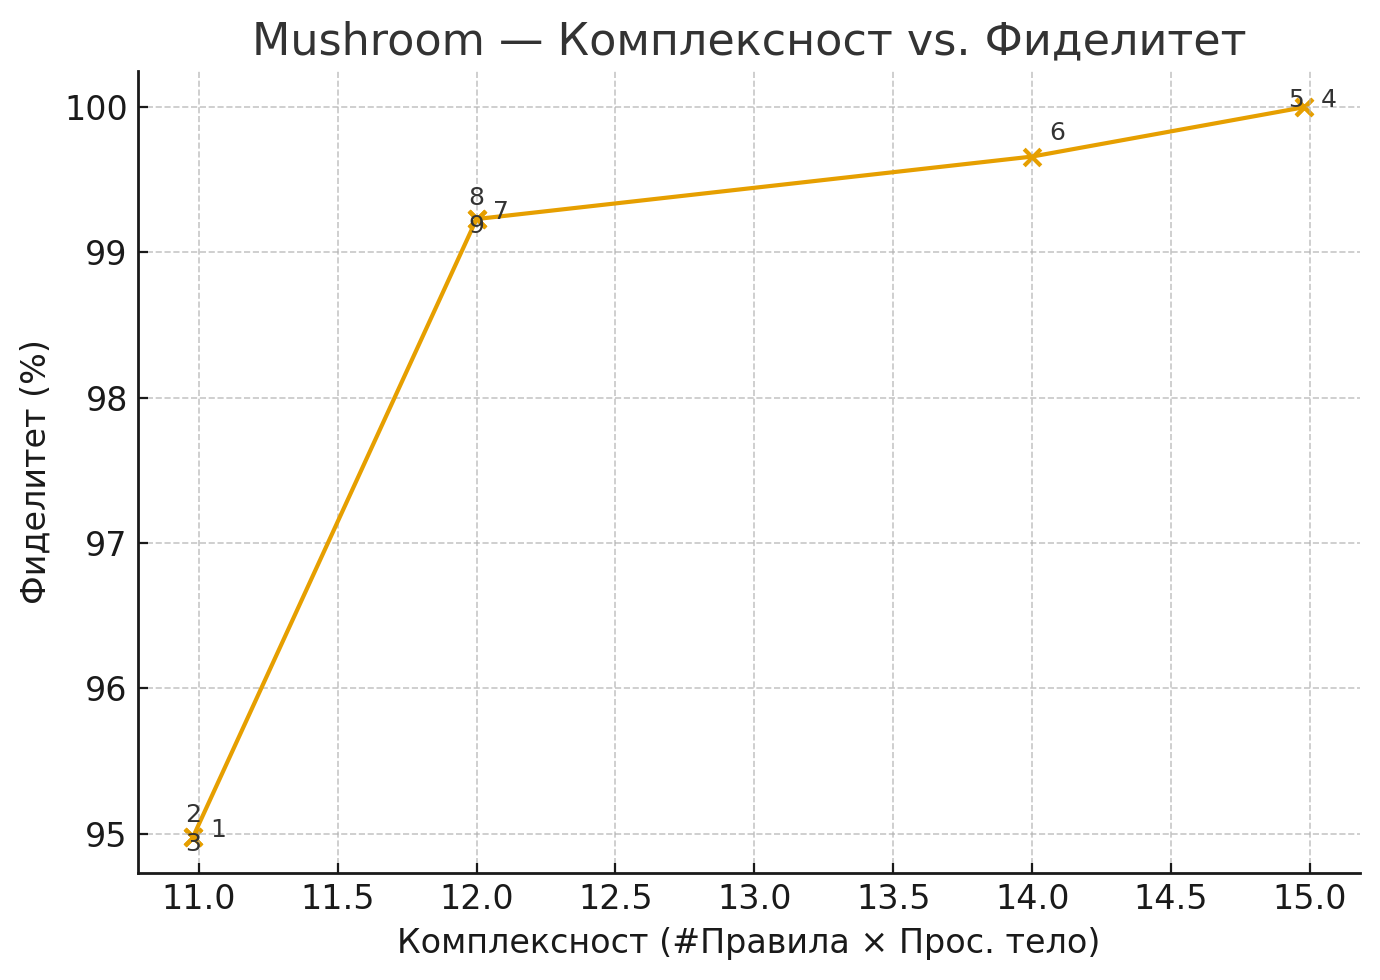
\includegraphics[width=.85\linewidth]{images/charts/mushroom-kompleksnost-fidelitet.png}
  \caption{Комплексност vs. Фиделитет — \textit{mushroom}.}
  \label{fig:mush-complexity-fidelity}
\end{figure}

Све тачке постижу веома високу тачност, преко 96\%. Ово додатно потврђује да је скуп \textit{mushroom} лако раздвојив, те да чак и једноставни модели могу постићи скоро савршене резултате. Као и код фиделитета, Парето фронт показује да се већ са врло једноставним моделима постиже максимум, па сложенији модели не доносе додатну вредност, видети слику \ref{fig:mush-complexity-accuracy}.
\begin{figure}[H]
  \centering
  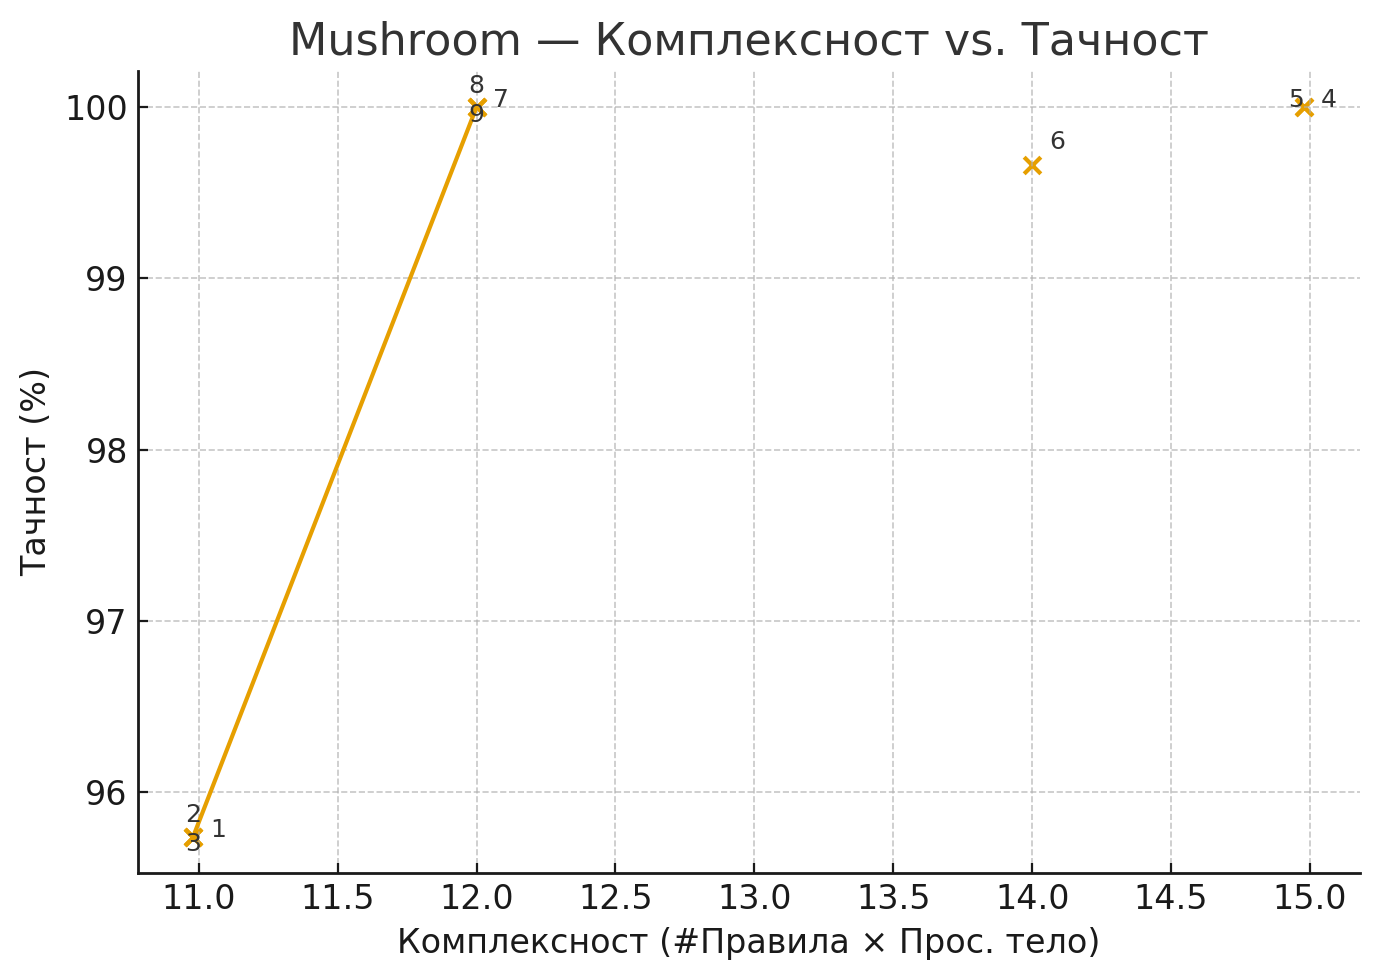
\includegraphics[width=.85\linewidth]{images/charts/mushroom-kompleksnost-tacnost.png}
  \caption{Комплексност vs. Тачност — \textit{mushroom}.}
  \label{fig:mush-complexity-accuracy}
\end{figure}

\textit{MCC} вредности су високе за све учитеље и све поставке, али \textit{DT} вредности су константно испод \textit{RF} и \textit{XGB}, што показује да ансамбл модели постижу бољу укупну корелацију предвиђања у односу на једноставније моделе, видети слику \ref{fig:mush-mcc}.
\begin{figure}[H]
  \centering
  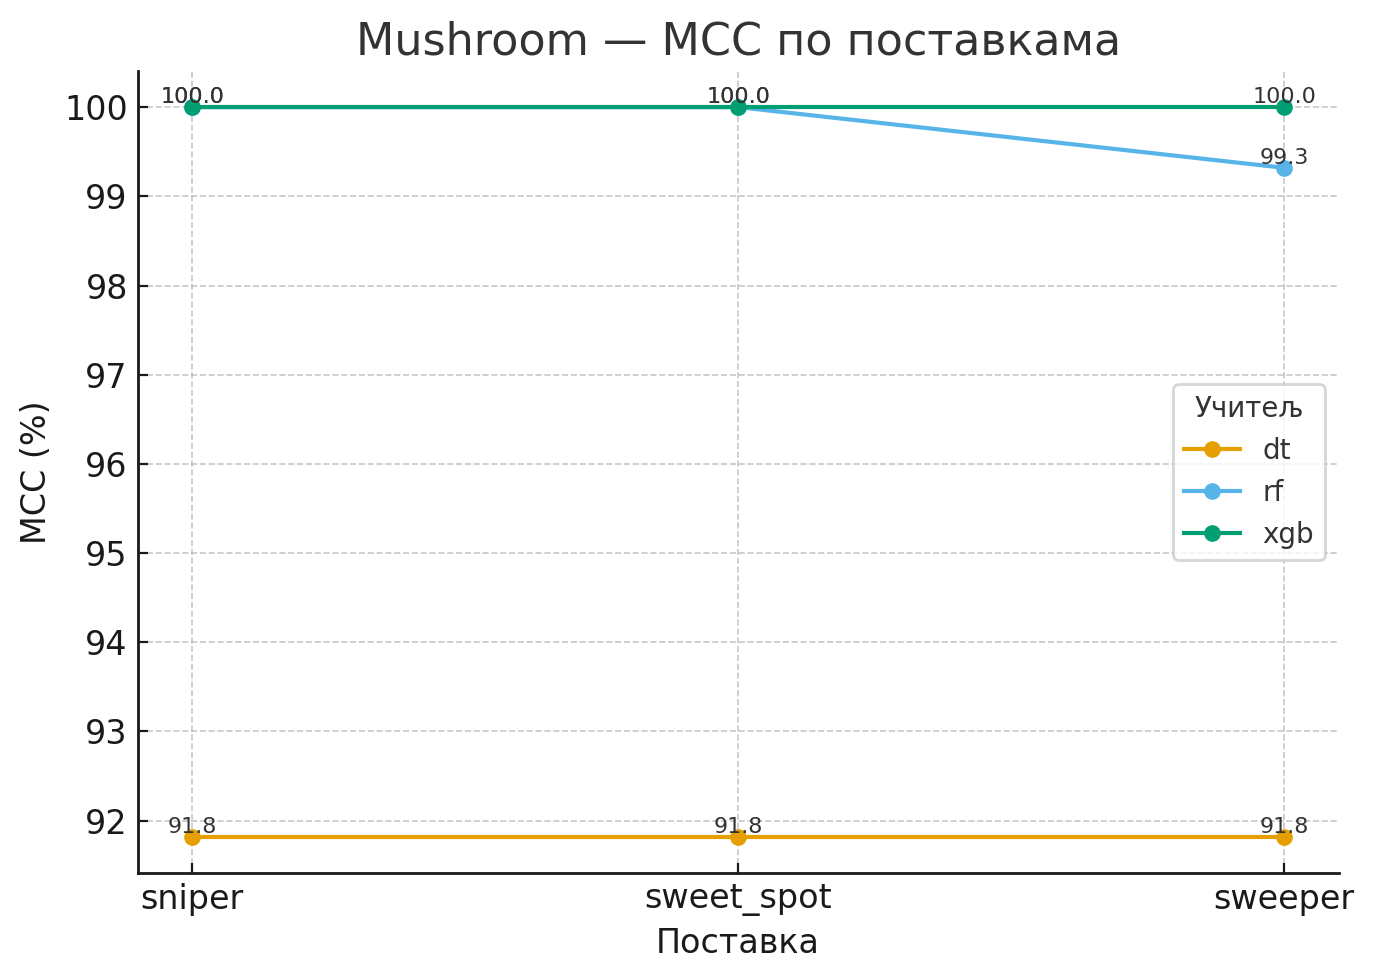
\includegraphics[width=.85\linewidth]{images/charts/mushroom-mcc.png}
  \caption{\textit{MCC} по поставкама — \textit{mushroom}.}
  \label{fig:mush-mcc}
\end{figure}

Табела \ref{tab:rules-top1-mushroom} приказује најбоље правило по комбинацији (датасет, учитељ, поставка). Правила су одабрана по највишој подршци.

\begin{table}[H]
\centering
\resizebox{\textwidth}{!}{
\begin{tabular}{@{}lllrrrrr@{}}
\toprule
\textbf{Скуп} & \textbf{Учитељ} & \textbf{Поставка} & \textbf{ИД правила} & \textbf{|Тело|} & \textbf{Подршка} & \textbf{Покривеност} & \textbf{Прецизност} \\
\midrule
mushroom & dt  & sniper     & 4  & 3 & 270 & 0.4530 & 1.0000 \\
mushroom & dt  & sweet\_spot& 4  & 3 & 270 & 0.4530 & 1.0000 \\
mushroom & dt  & sweeper    & 4  & 3 & 270 & 0.4530 & 1.0000 \\
mushroom & rf  & sniper     & 7  & 3 & 352 & 0.5997 & 1.0000 \\
mushroom & rf  & sweet\_spot& 7  & 3 & 352 & 0.5997 & 1.0000 \\
mushroom & rf  & sweeper    & 8  & 2 & 352 & 0.5997 & 1.0000 \\
mushroom & xgb & sniper     & 8  & 1 & 332 & 0.5589 & 1.0000 \\
mushroom & xgb & sweet\_spot& 8  & 1 & 332 & 0.5589 & 1.0000 \\
mushroom & xgb & sweeper    & 8  & 1 & 332 & 0.5589 & 1.0000 \\
\bottomrule
\end{tabular}
}
\caption{Најбоље правило за скуп \textit{mushroom} по комбинацији (учитељ, поставка), бирано по највишој подршци.}
\label{tab:rules-top1-mushroom}
\end{table}

Уочава се висока стабилност и понављање истих клауза кроз различите поставке и учитеље. Код \textit{DT} учитеља идентична тролитерална клауза $spore\_print\_color = white \land ring\_number = one \land gill\_spacing = close$ доследно се јавља у \textit{sniper}, \textit{sweet\_spot} и \textit{sweeper} поставкама са истом подршком (270) и прецизношћу (1.00). Код \textit{XGB} учитеља једнолитерална клауза $odor = foul$ понавља се у све три поставке (подршка 332, прецизност 1.00). Код \textit{RF} учитеља тролитерална клауза се јавља у \textit{sniper} и \textit{sweet\_spot}, док се у \textit{sweeper} поставци појављује њена редукована дволитерална верзија са истом подршком (352) и прецизношћу (1.00).

Ови налази указују на постојање врло чистих сепаратора класа, чија се структура мало мења са променом поставке. Разлике међу учитељима огледају се у избору атрибута: \textit{DT} фаворизује $spore\_print$ карактеристике, \textit{RF} физичке особине (нпр. модрице, површина), док \textit{XGB} даје приоритет мирису.

\paragraph{Напомена о наредним графиконима} У наредним графиконима, за сваку метрику, приказане су вредности у односу на учитеља и истину по свим комбинацијама учитељ/поставка. За сваку метрику приказан је засебан графикон.

Тачност према истини је једнака или незнатно виша од тачности према учитељу, многе комбинације су практично савршене. Ово указује да дестилат постиже бар онолико исправних предвиђања према истини колико и усклађених предвиђања са учитељем. Видети слику \ref{fig:mush-acc}.
\begin{figure}[H]
  \centering
  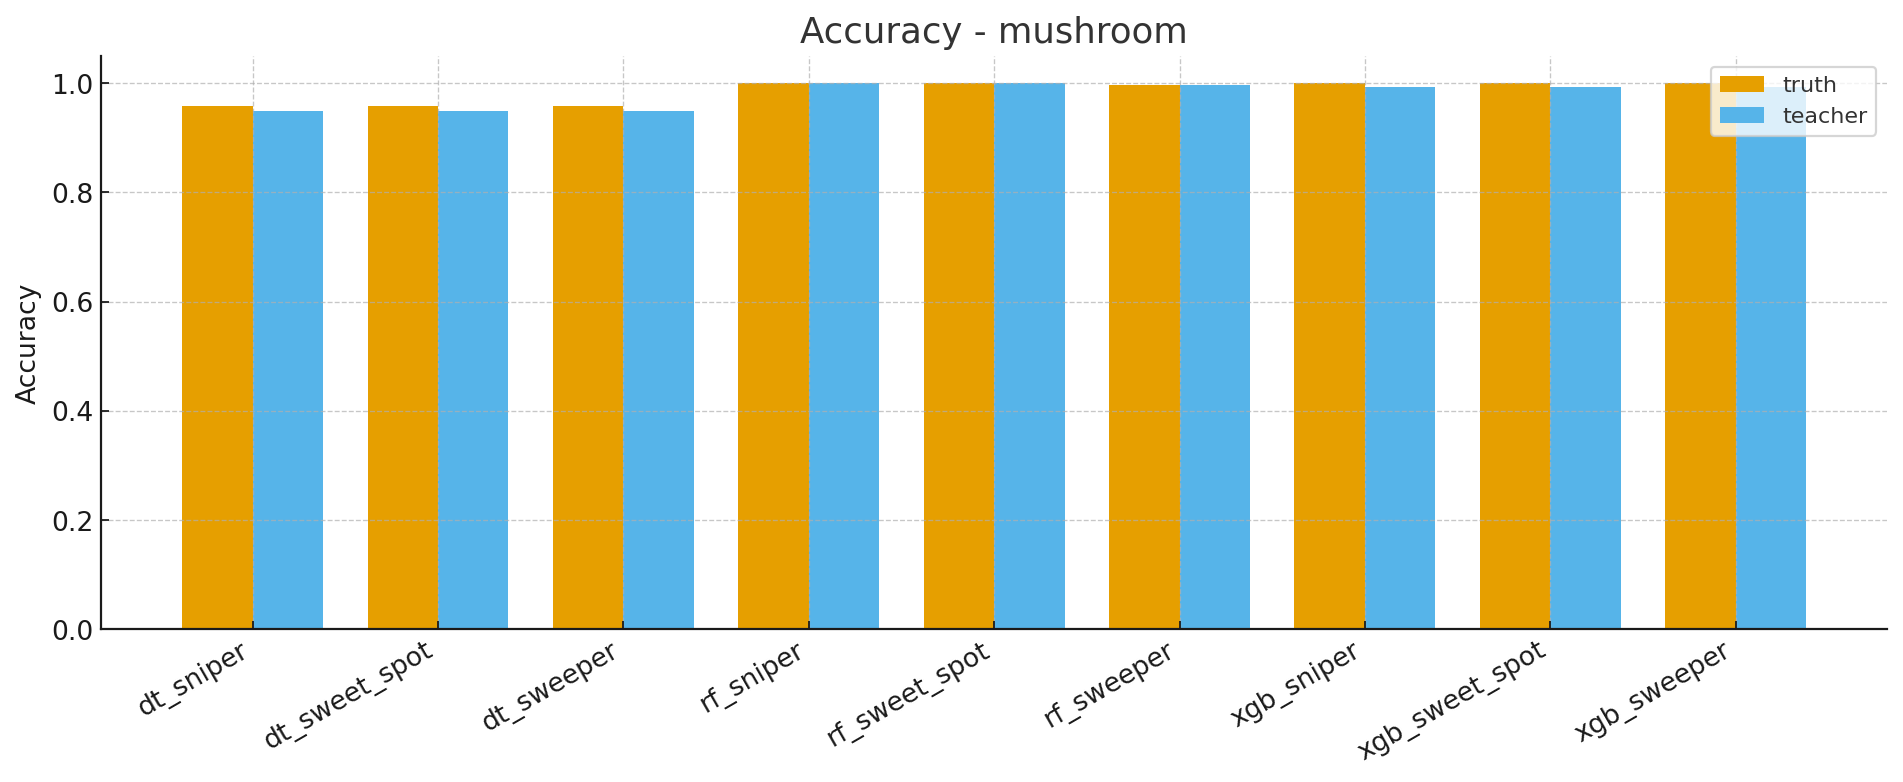
\includegraphics[width=.85\linewidth]{images/charts/accuracy_simple_mushroom.png}
  \caption{Accuracy — \textit{mushroom}.}
  \label{fig:mush-acc}
\end{figure}

Скоро све вредности су 1.0 (или врло близу) и према истини и према учитељу, позитивне прогнозе су истовремено коректне и усклађене са учитељем, уз минималне разлике. Видети слику \ref{fig:mush-prec}.
\begin{figure}[H]
  \centering
  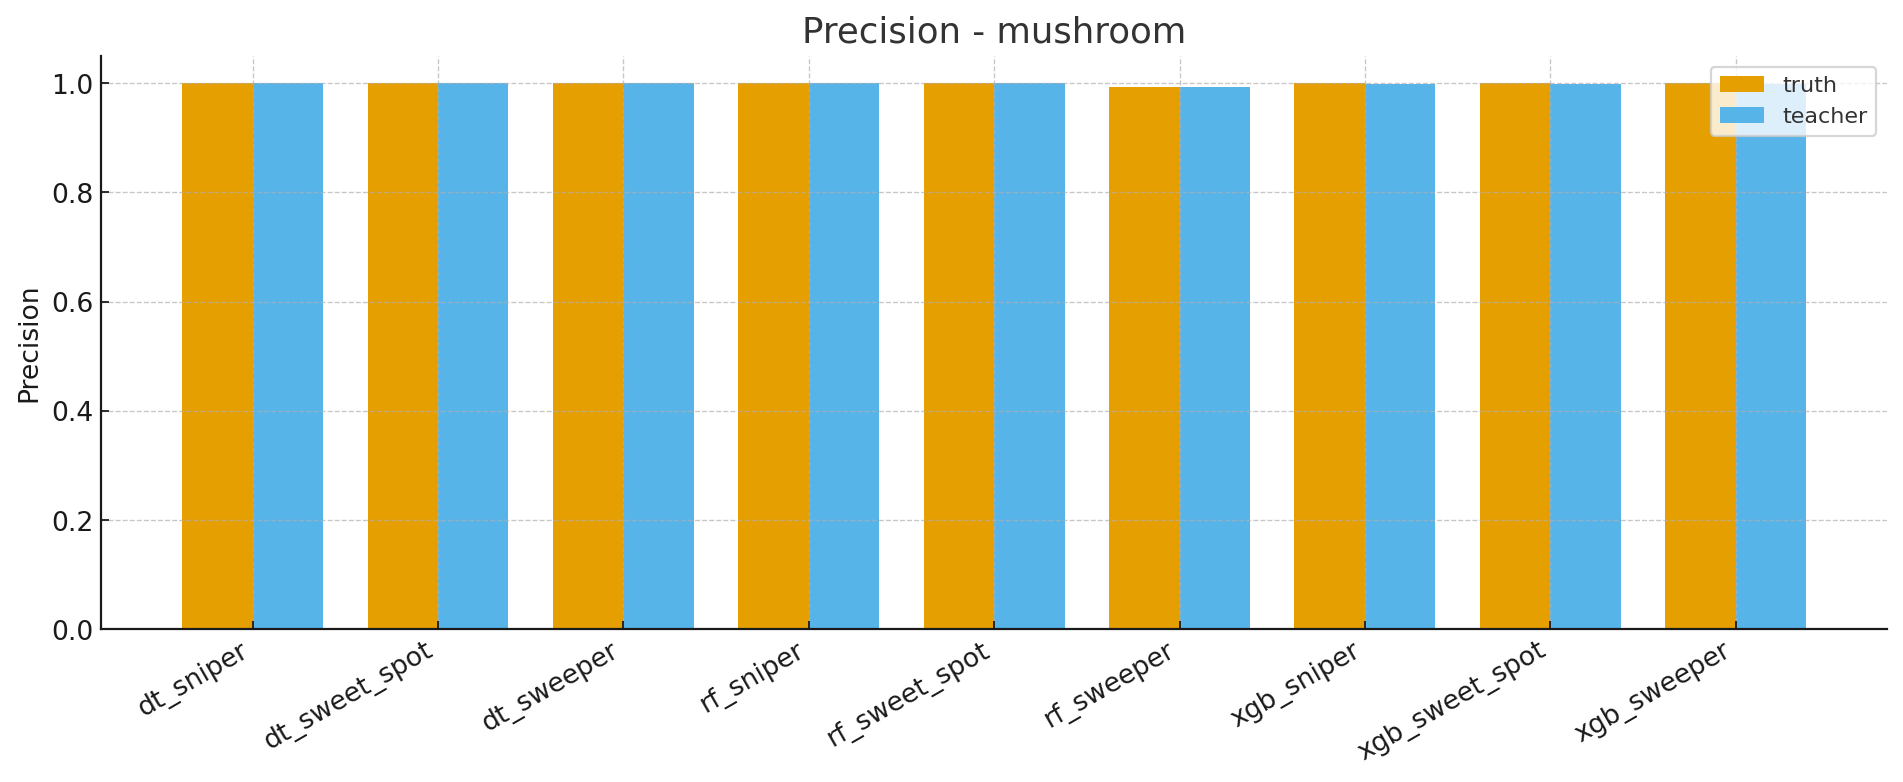
\includegraphics[width=.85\linewidth]{images/charts/precision_simple_mushroom.png}
  \caption{Precision — \textit{mushroom}.}
  \label{fig:mush-prec}
\end{figure}

Одзив према истини је једнак или нешто већи од одзива према учитељу (а за \texttt{rf} практично савршен у оба режима), што показује да дестилат идентификује готово све стварне позитиве и да га учитељев скуп позитивних примера не „ограничава“. Видети слику \ref{fig:mush-recall}.
\begin{figure}[H]
  \centering
  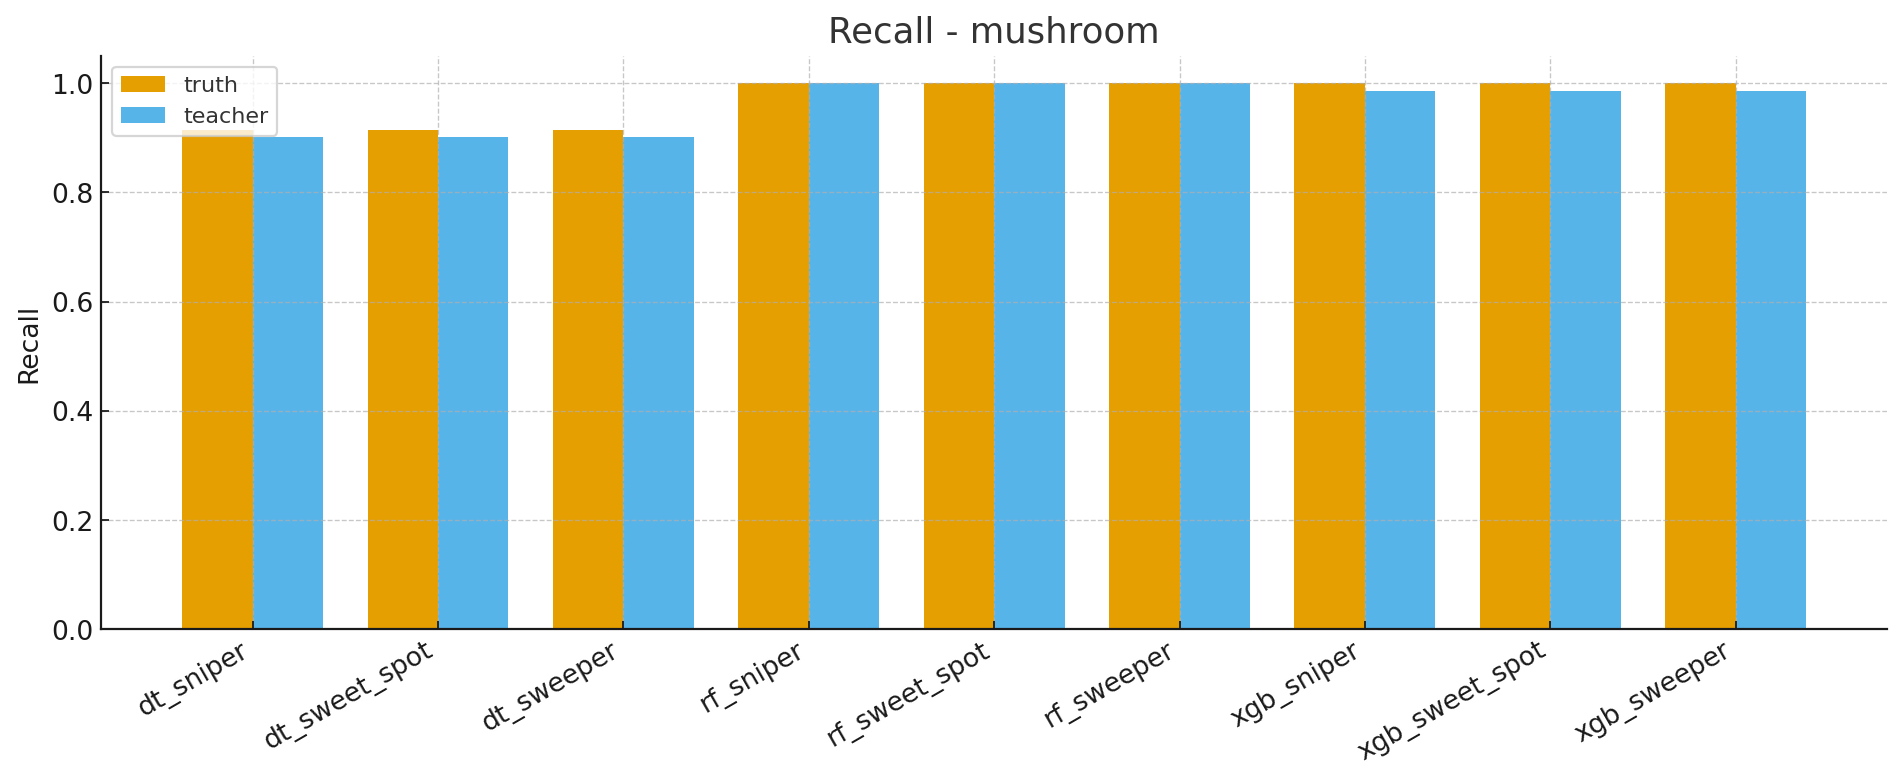
\includegraphics[width=.85\linewidth]{images/charts/recall_simple_mushroom.png}
  \caption{Recall — \textit{mushroom}.}
  \label{fig:mush-recall}
\end{figure}

F1 према истини је једнак или незнатно виши од F1 према учитељу (за \texttt{rf} савршен у оба), што значи да је стварни баланс прецизности и одзива најмање онолико добар колико и верност учитељу, још један показатељ перформанси које су близу максимума. Видети слику \ref{fig:mush-f1}.
\begin{figure}[H]
  \centering
  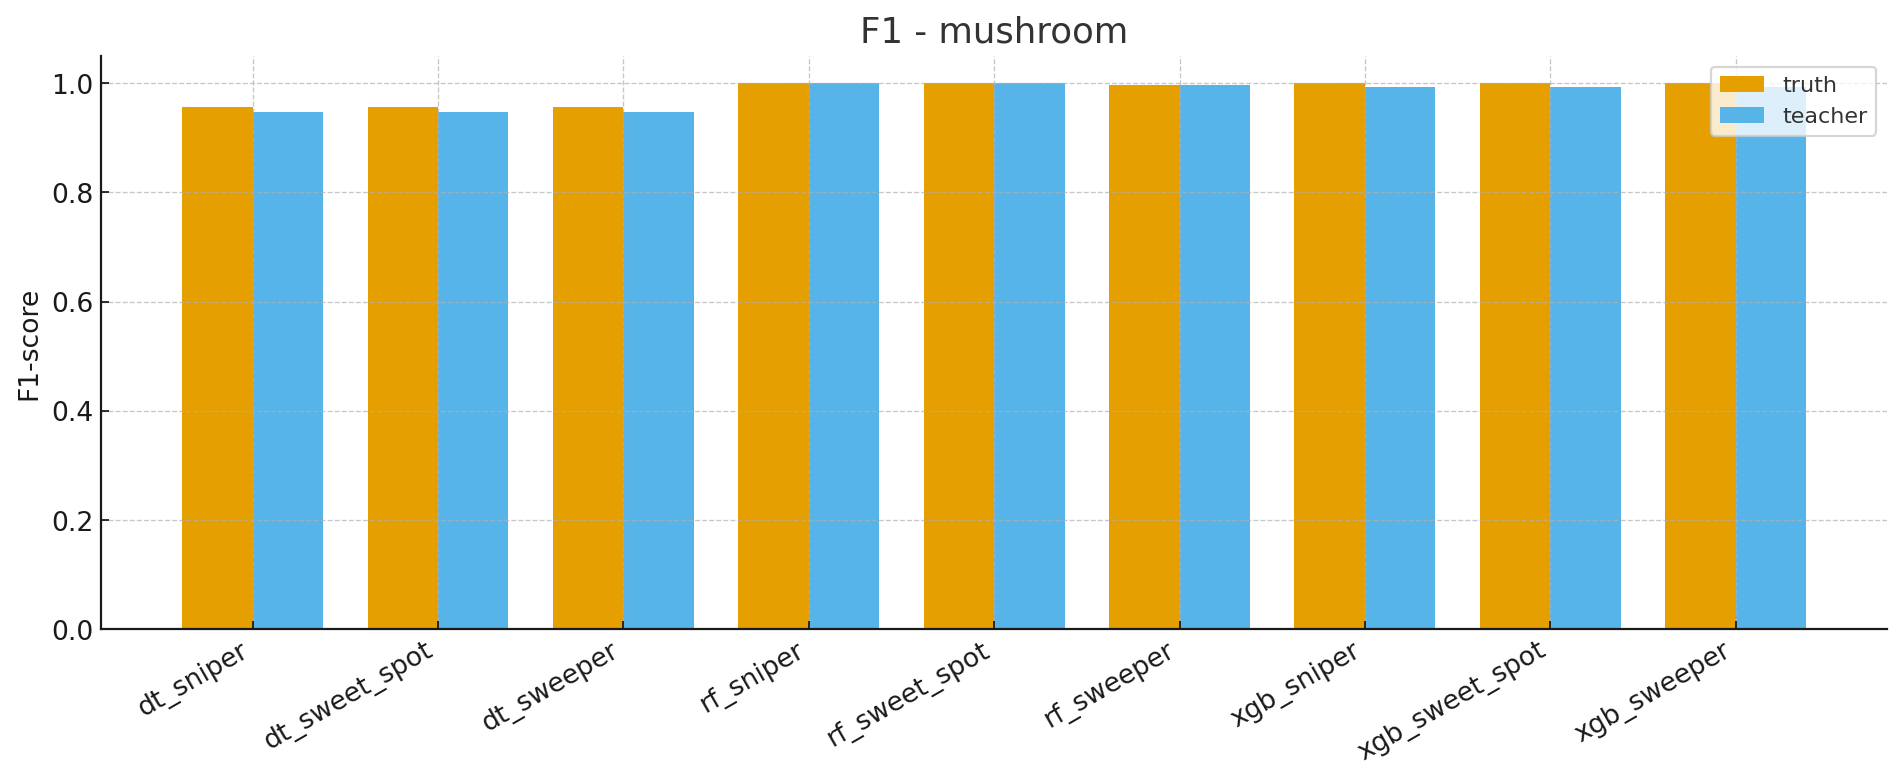
\includegraphics[width=.85\linewidth]{images/charts/f1_simple_mushroom.png}
  \caption{F1 — \textit{mushroom}.}
  \label{fig:mush-f1}
\end{figure}

\textit{MCC} према истини је једнак или нешто виши од \textit{MCC} према учитељу (за \texttt{rf} ≈ 1.0 у оба), што говори да је глобална усаглашеност са истинитим ознакама барем толико добра као и са учитељем, практично максимум перформанси на овом скупу. Видети слику \ref{fig:mush-mcc-tt}.
\begin{figure}[H]
  \centering
  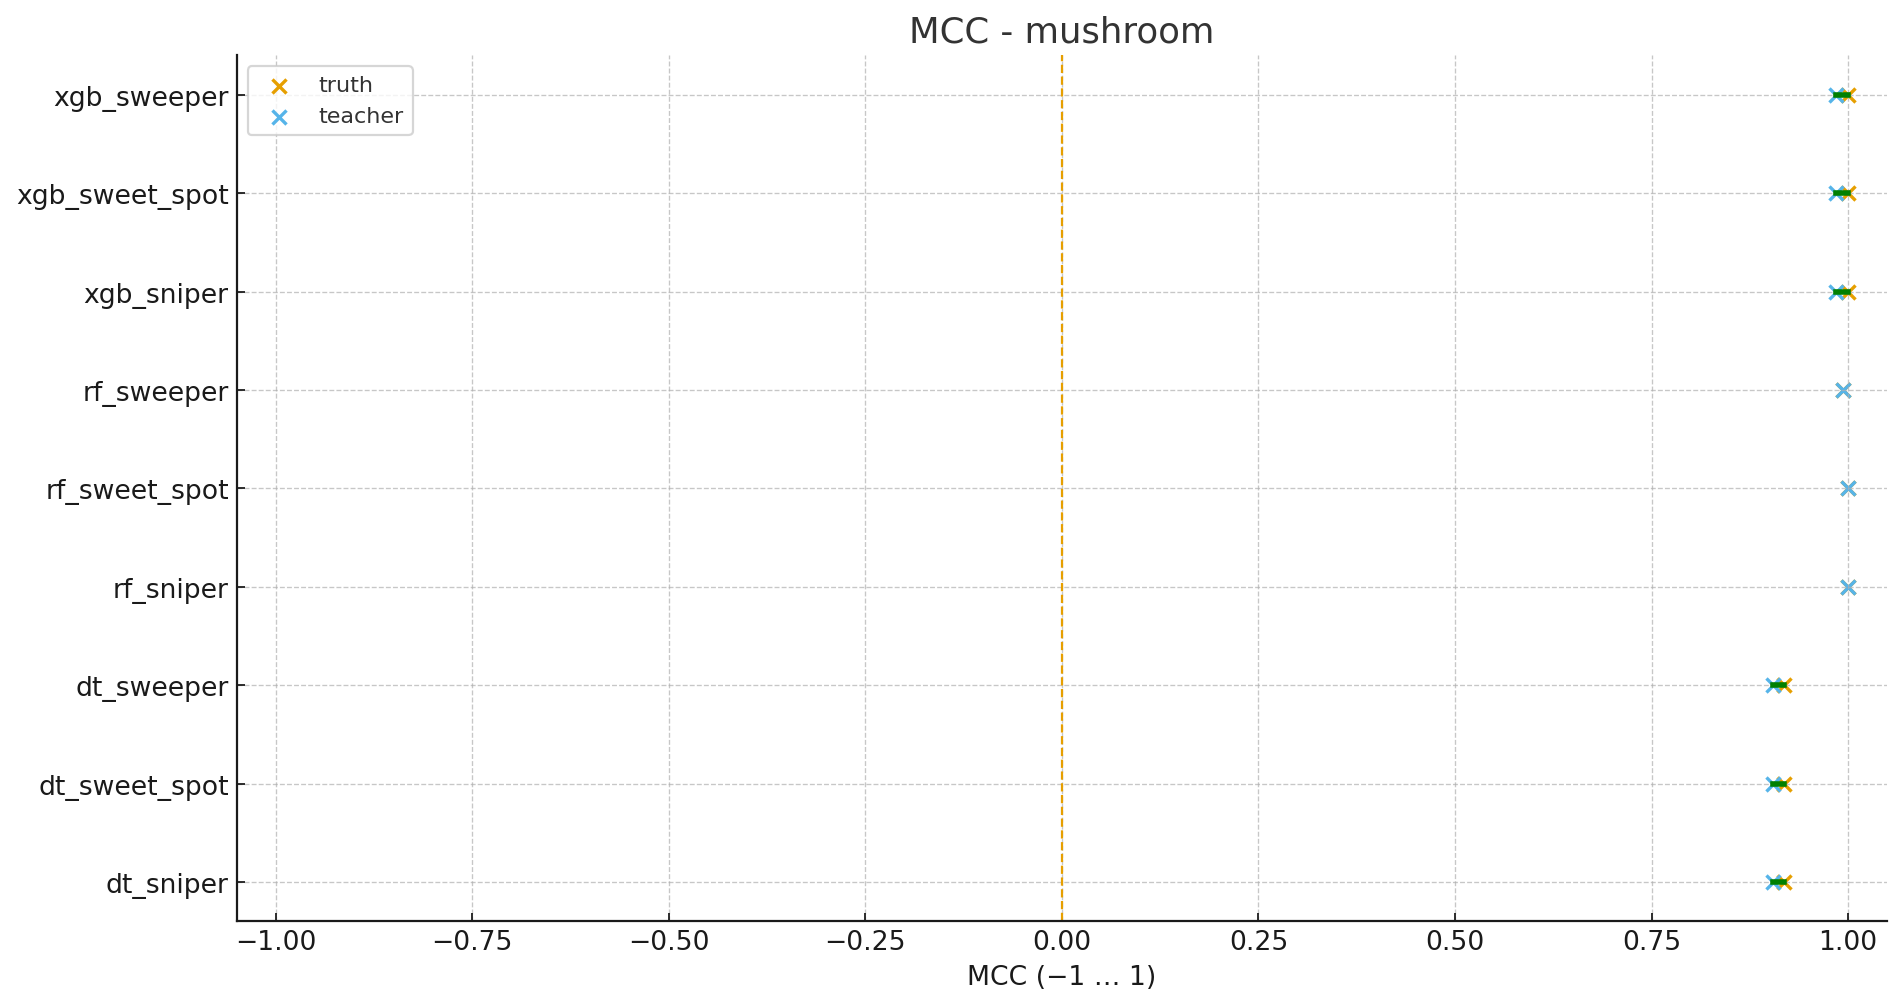
\includegraphics[width=.85\linewidth]{images/charts/mcc_simple_mushroom.png}
  \caption{\textit{MCC} — \textit{mushroom}.}
  \label{fig:mush-mcc-tt}
\end{figure}

\subsubsection*{Закључак — \textit{mushroom}}
На скупу \textit{mushroom} дестилација у Aleph-у даје готово савршене моделе: фиделитет је стабилно ≥95\%, а тачност ≥96\% у свим пресетима и за све учитеље. Парето анализа показује „колено“ већ при малом броју правила и кратким телима клауза, а додатна сложеност не доноси добит. \textit{MCC} је висок за све, при чему \textit{RF}/\textit{XGB} благо надмашују \textit{DT}. Најбоља правила су изузетно стабилна преко пресета (нпр. једнолитерално \texttt{odor=foul} код \textit{XGB}, \textit{spore print} карактеристике код \textit{DT}, физичке особине код \textit{RF}), што потврђује постојање „чистих“ сепаратора класа. Перформансе према истини су једнаке или незнатно више од перформанси према учитељу, па је дестилат и веродостојан и коректан. Практично, препоручљиве су једноставније поставке (\texttt{heuristic} претрага, мањи \texttt{clauselength}, конзервативан \texttt{minacc}, низак \texttt{noise}). Овај скуп је, дакле, лако раздвојив и омогућава максималну објашњивост без губитка квалитета.


%%% ADULT %%%
\subsubsection{Adult}

У табели \ref{tab:aleph-adult} су приказана Aleph подешавања за скуп \textit{adult}, која варирају у зависности од учитељског модела и поставке.

\begin{table}[H]
\centering
\small
\setlength{\tabcolsep}{3pt}
\begin{tabularx}{\textwidth}{@{} l l c c c c c c c c @{}}
\toprule
\textbf{Учитељ} & \textbf{Поставка} & \texttt{search} & \texttt{openlist} & \texttt{nodes} & \texttt{evalfn} & \texttt{cl} & \texttt{minacc} & \texttt{minpos} & \texttt{noise} \\
\midrule
dt  & sniper      & heuristic & 60   & 100k & laplace  & 4 & 0.80 & 5 & 200  \\
dt  & sweet\_spot & heuristic & 80   & 120k & wracc    & 3 & 0.70 & 5 & 400  \\
dt  & sweeper     & bf        & 1500 & 200k & coverage & 2 & 0.60 & 5 & 1400 \\
rf  & sniper      & heuristic & 60   & 100k & laplace  & 6 & 0.80 & 5 & 200  \\
rf  & sweet\_spot & heuristic & 80   & 120k & wracc    & 4 & 0.70 & 5 & 400  \\
rf  & sweeper     & bf        & 1500 & 200k & coverage & 3 & 0.60 & 5 & 1400 \\
xgb & sniper      & heuristic & 60   & 100k & laplace  & 6 & 0.80 & 5 & 200  \\
xgb & sweet\_spot & heuristic & 80   & 120k & wracc    & 4 & 0.70 & 5 & 400  \\
xgb & sweeper     & bf        & 1500 & 200k & coverage & 3 & 0.60 & 5 & 1400 \\
\bottomrule
\caption{Aleph подешавања за \textit{adult} по учитељу и поставци. Напомена: \texttt{cl} означава \texttt{clauselength}.}
\label{tab:aleph-adult}
\end{tabularx}
\end{table}

%OVDE
\paragraph{Резултати} Табела \ref{tab:ilp-adult} приказује перформансе дестилованих ИЛП модела у односу на сложеност, са метрикама као што су тачност (accuracy), \textit{MCC}, фиделитет, број правила и просечна дужина тела правила. На дијаграмима расејања су поједини записи означени својим \emph{ID}-јем, који се може наћи у табели.

Повећање комплексности побољшава фиделитет, али ефекат се брзо смањује, јер после одређене тачке раст броја правила и дужине тела не доноси значајно бољи резултат, Парето фронт омогућава да се идентификују оптималне конфигурације које балансирају квалитет и једноставност. Све поставке сем \texttt{sweeper} дају резултате који имају фиделитет \textit{> 0.75}. Видети слику \ref{fig:adult-complexity-fidelity}.
\begin{figure}[H]
  \centering
  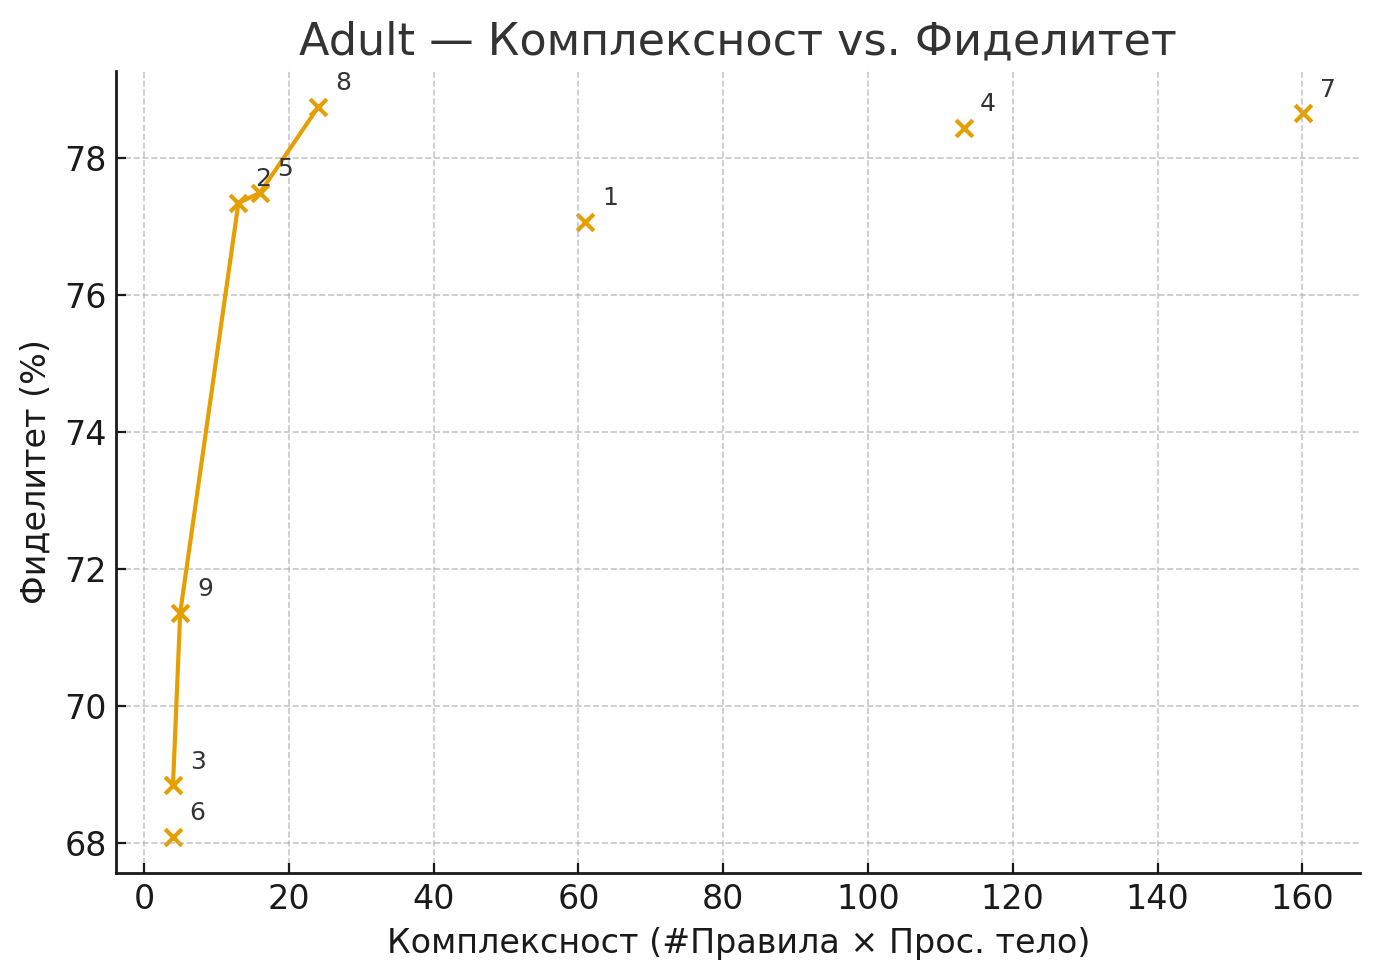
\includegraphics[width=.85\linewidth]{images/charts/adult-kompleksnost-fidelitet.png}
  \caption{Комплексност vs. Фиделитет — \textit{adult}.}
  \label{fig:adult-complexity-fidelity}
\end{figure}

Као и код фиделитета, већа комплексност донекле побољшава тачност, али добици после одређене тачке постају занемарљиви, Парето фронт помаже да се изабере модел који нуди најбољи однос тачности и једноставности, слично као код фиделитета, где све поставке сем \texttt{sweeper} дају резултате који имају тачност \textit{> 0.74}. Видети слику \ref{fig:adult-complexity-accuracy}.
\begin{figure}[H]
  \centering
  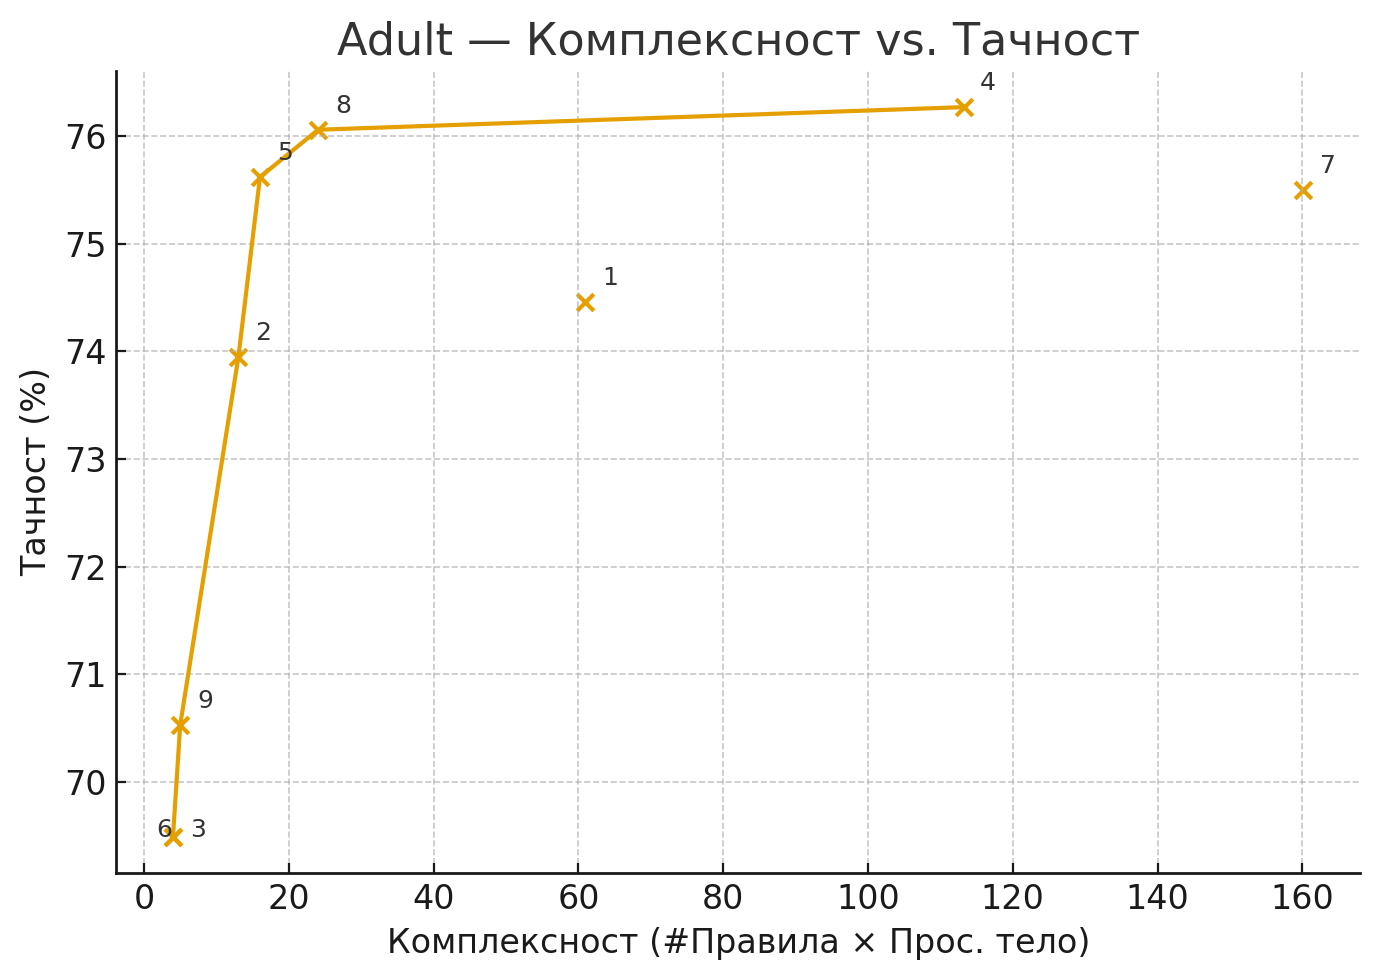
\includegraphics[width=.85\linewidth]{images/charts/adult-kompleksnost-tacnost.png}
  \caption{Комплексност vs. Тачност — \textit{adult}.}
  \label{fig:adult-complexity-accuracy}
\end{figure}

Постоји јасно опадање \textit{MCC} при преласку са \textit{sniper} на \textit{sweeper} поставке, што значи да смањивање комплексности доводи до губитка квалитета, а \textit{sniper} и \textit{sweet\_spot} дају најбољи резултат. Такође, \textit{DT} учитељ даје конзистентно најнижи \textit{MCC}, док \textit{RF} и \textit{XGB} дају сличне и боље резултате, што указује на предност ансамбл модела у овом случају. Видети слику \ref{fig:adult-mcc}.
\begin{figure}[H]
  \centering
  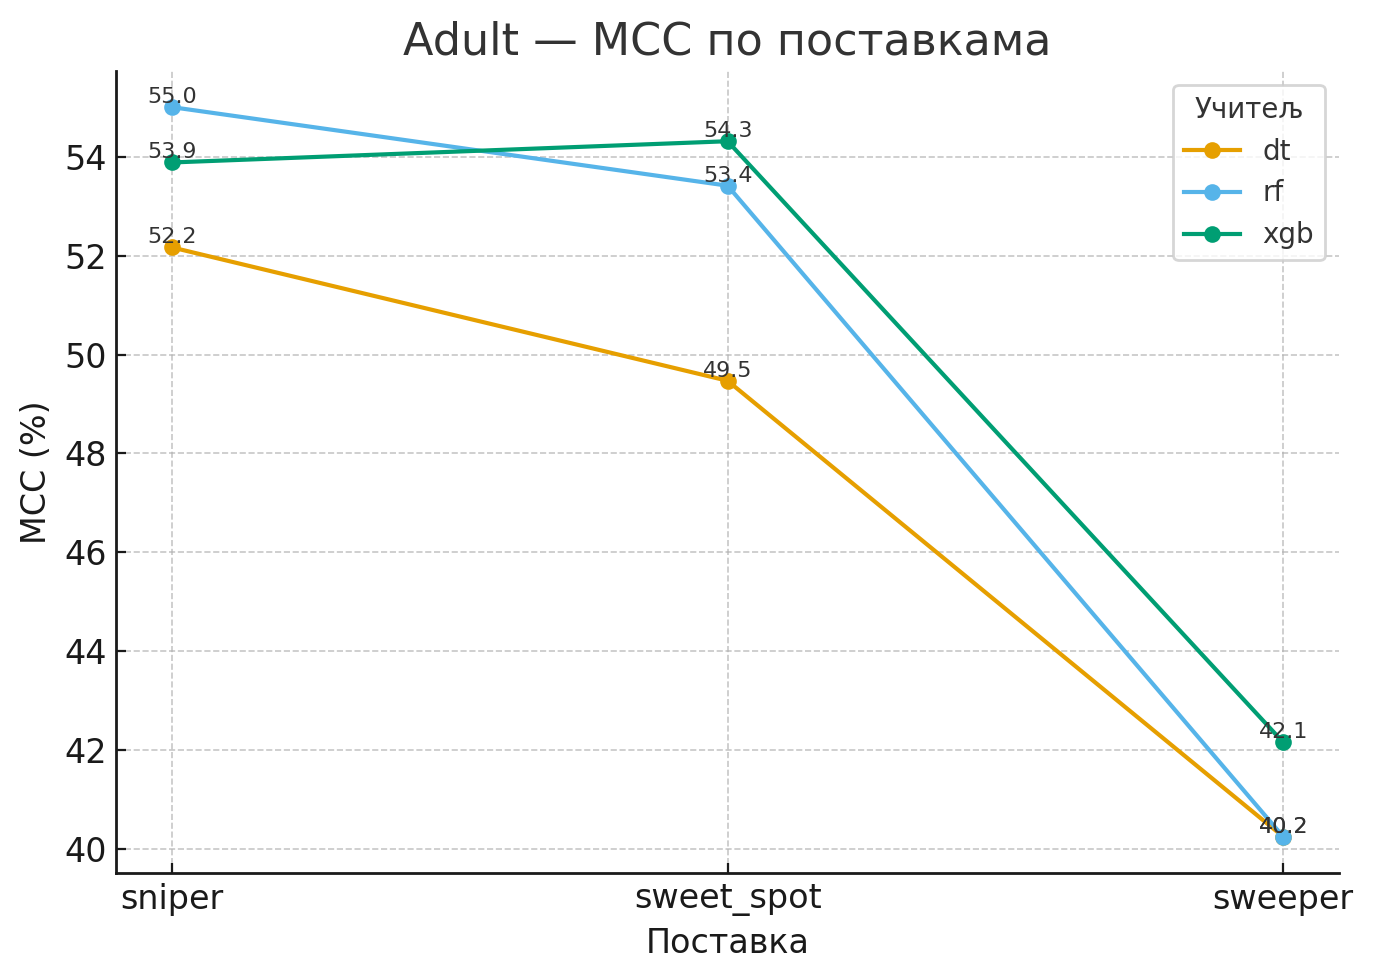
\includegraphics[width=.85\linewidth]{images/charts/adult-mcc.png}
  \caption{\textit{MCC} по поставкама — \textit{adult}.}
  \label{fig:adult-mcc}
\end{figure}

Табела \ref{tab:rules-top1-adult} приказује најбоље правило по комбинацији (датасет, учитељ, поставка). Правила су одабрана по највишој подршци.

\begin{table}[H]
\centering
\resizebox{\textwidth}{!}{
\begin{tabular}{@{}lllrrrrr@{}}
\toprule
\textbf{Скуп} & \textbf{Учитељ} & \textbf{Поставка} & \textbf{ИД правила} & \textbf{|Тело|} & \textbf{Подршка} & \textbf{Покривеност} & \textbf{Прецизност} \\
\midrule
adult    & dt  & sniper     & 19 & 3 & 174 & 0.0943 & 1.0000 \\
adult    & dt  & sweet\_spot& 3  & 1 & 196 & 0.1062 & 1.0000 \\
adult    & dt  & sweeper    & 2  & 1 & 196 & 0.1062 & 1.0000 \\
adult    & rf  & sniper     & 38 & 2 & 294 & 0.1565 & 1.0000 \\
adult    & rf  & sweet\_spot& 8  & 2 & 294 & 0.1565 & 1.0000 \\
adult    & rf  & sweeper    & 2  & 1 & 196 & 0.1033 & 0.9898 \\
adult    & xgb & sniper     & 52 & 3 & 220 & 0.1211 & 1.0000 \\
adult    & xgb & sweet\_spot& 11 & 2 & 294 & 0.1591 & 0.9830 \\
adult    & xgb & sweeper    & 2  & 1 & 196 & 0.1068 & 0.9898 \\
\bottomrule
\end{tabular}
}
\caption{Најбоље правило за скуп \textit{adult} по комбинацији (учитељ, поставка), бирано по највишој подршци.}
\label{tab:rules-top1-adult}
\end{table}

За скуп adult доминира нешто већа разноврсност издвојених правила. Једнолитерална клауза $capital\_gain=medium$ појављује се као најбоље у више учитеља и поставки, што указује на њену робусност као индикатора класе. Клауза $education=advanced\_degree \land marital\_status=married\_civ\_spouse$ доследно се јавља код \textit{RF} учитеља (\textit{sniper}, \textit{sweet\_spot}) и код \textit{XGB} учитеља (\textit{sweet\_spot}) са идентичном подршком, што потврђује њен значај за предвиђање високе зараде.

Поставке \textit{sniper} чешће фаворизују тролитералне клаузе мање покривености али веће специфичности (нпр. \textit{XGB}: $bachelors \land married \land hours>40$, \textit{DT}: $husband \land bachelors \land age\ 35–45$), док \textit{sweet\_spot} и \textit{sweeper} поставке преферирају једноставније клаузе шире примене, при чему прецизност зависи од самог атрибута, поједина једнолитерална правила као што је $capital\_gain = medium$ задржавају веома високу прецизност, док друга имају умерену.


Уочава се да више учитеља и поставки конзистентно издваја исте једно- или дволитералне клаузе, што указује на постојање стабилних и интерпретабилних правила, док комплексније клаузе омогућавају додавање специфичних услова који повећавају прецизност у ужим подскуповима података.

\paragraph{Напомена о наредним графиконима} У наредним графиконима, за сваку метрику, приказане су вредности у односу на учитеља и истину по свим комбинацијама учитељ/поставка. За сваку метрику приказан је засебан графикон.


На adult сету тачност према учитељу је у већини случајева виша од тачности према истини, што значи да дестилат чешће погађа учитељеве ознаке него што је заиста у праву, у \textit{sweeper} конфигурацијама се ово понекад преокреће, али доминира образац \emph{фиделитет > стварна тачност}. Претпоставка је да је учитељ увео одређену дозу шума у ознаке, коју дестилат довољно успешно имитира, али која смањује стварни квалитет. Видети слику \ref{fig:adult-acc}.
\begin{figure}[H]
  \centering
  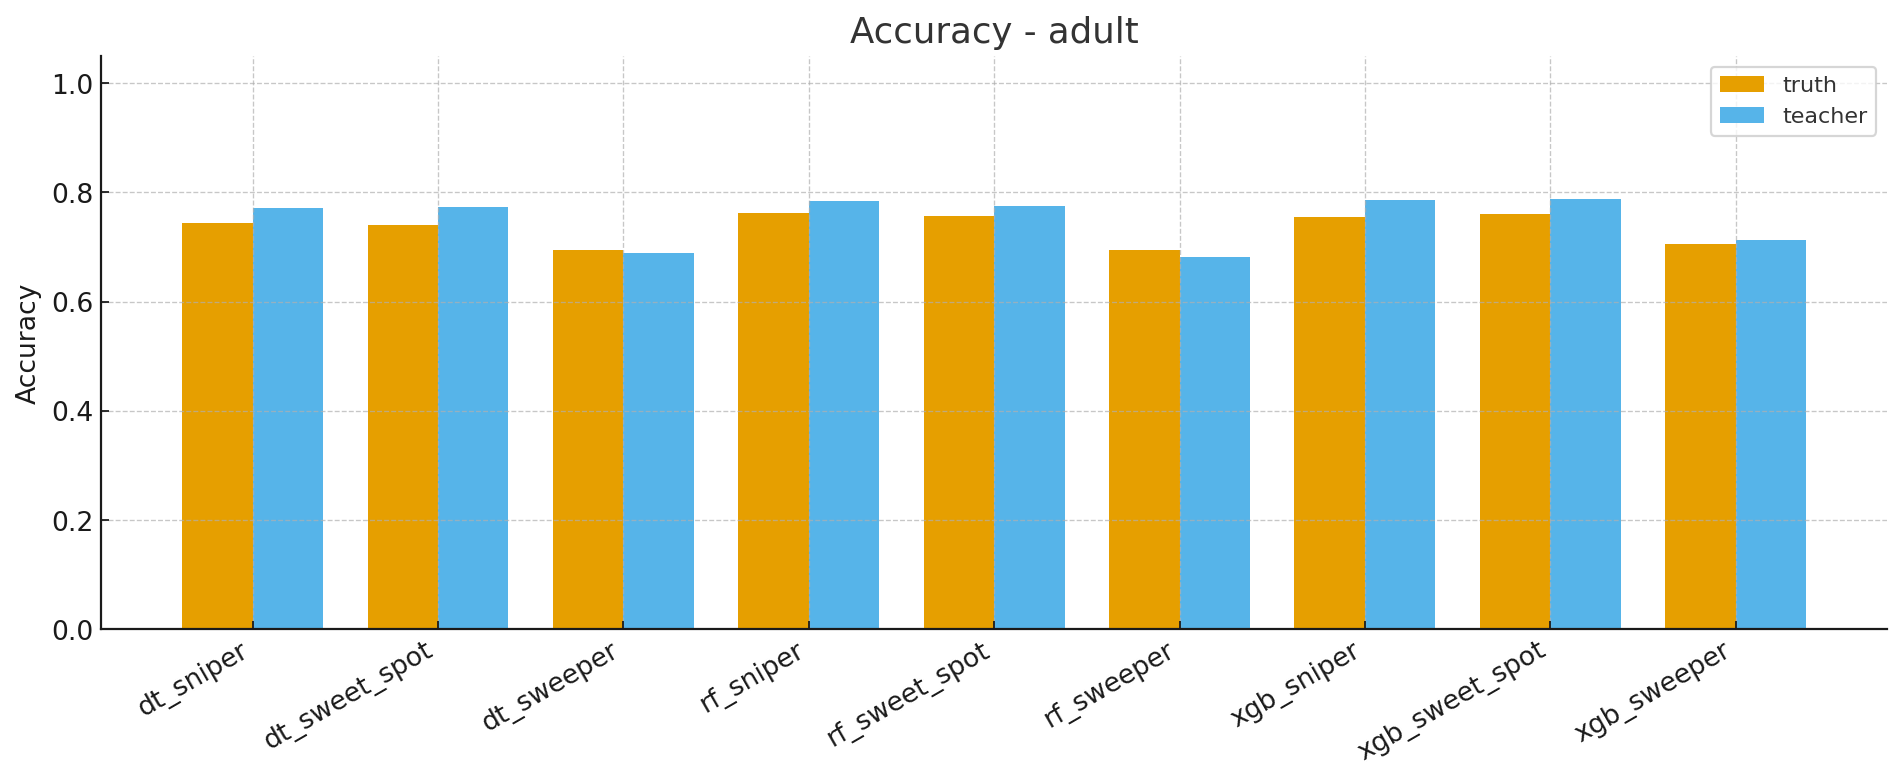
\includegraphics[width=.85\linewidth]{images/charts/accuracy_simple_adult.png}
  \caption{Accuracy — \textit{adult}.}
  \label{fig:adult-acc}
\end{figure}

Прецизност према учитељу је знатно виша од прецизности према истини у свим поставкама/моделима: када дестилат прогнозира „позитивно“, то се врло често поклапа са учитељем, али ређе са истинитим ознакама, висока верност позитивима учитеља, уз мању реалну прецизност. Опет, претпоставка је да учитељеве ознаке садрже шум који дестилат имитира, али генерализација није довољно добра. Видети слику \ref{fig:adult-acc}.
\begin{figure}[H]
  \centering
  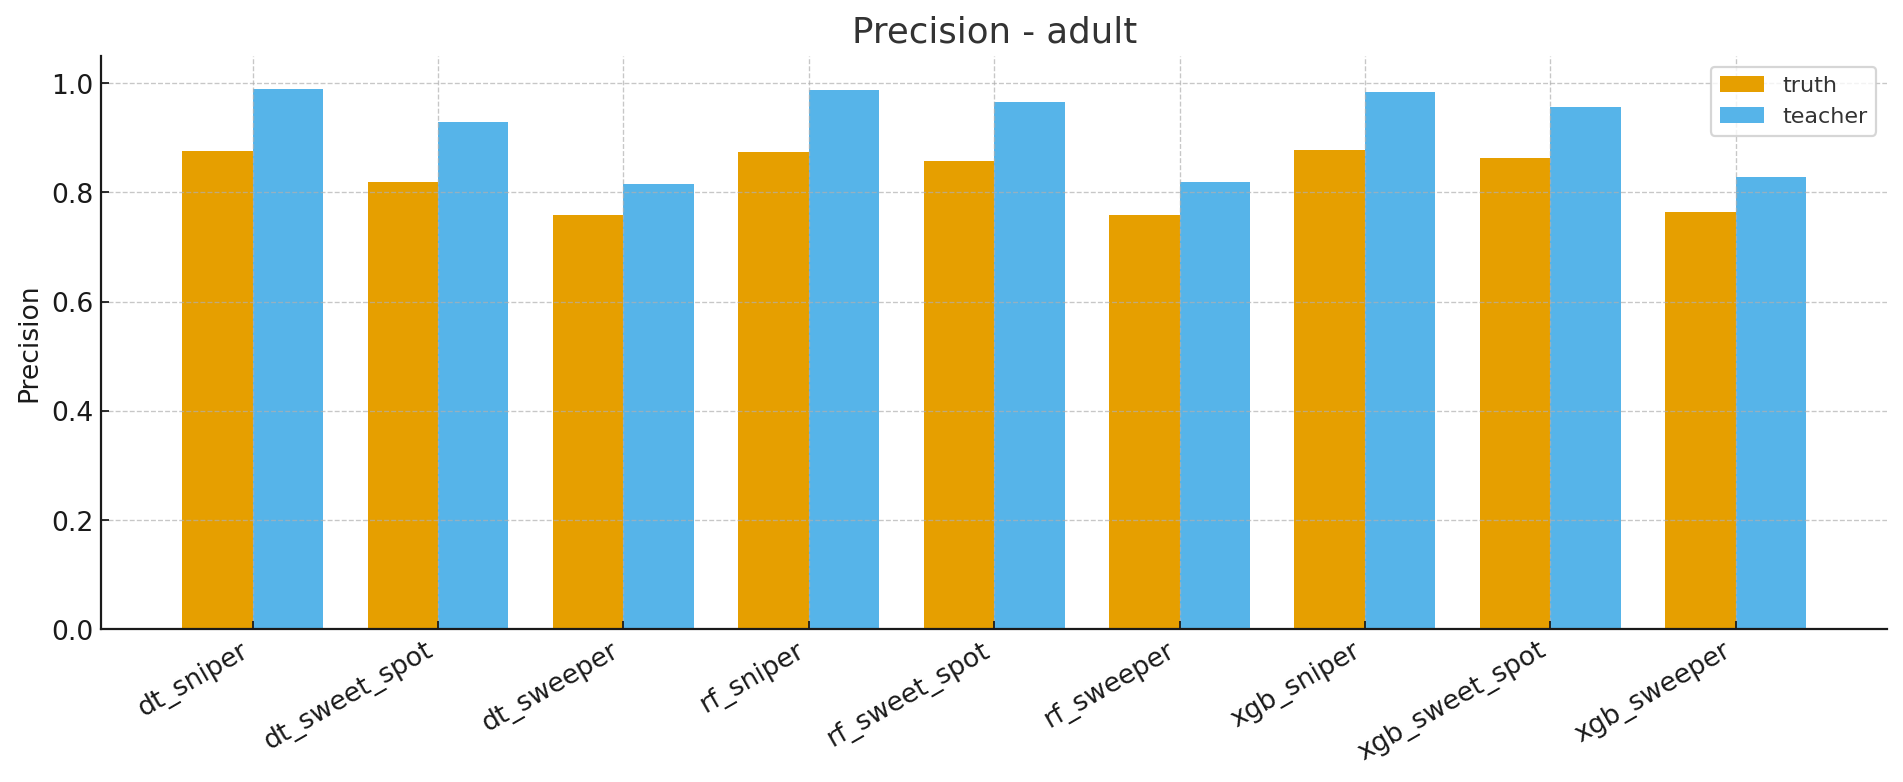
\includegraphics[width=.85\linewidth]{images/charts/precision_simple_adult.png}
  \caption{Precision — \textit{adult}.}
  \label{fig:adult-prec}
\end{figure}

Одзив према учитељу је у већини случајева мало већи или сличан одзиву према истини, што значи да дестилат боље „покрива“ учитељеве позитиве него стварне позитиве, у \textit{sweeper} поставкама одзив може пасти испод одзива према истини. Видети слику \ref{fig:adult-recall}.
\begin{figure}[H]
  \centering
  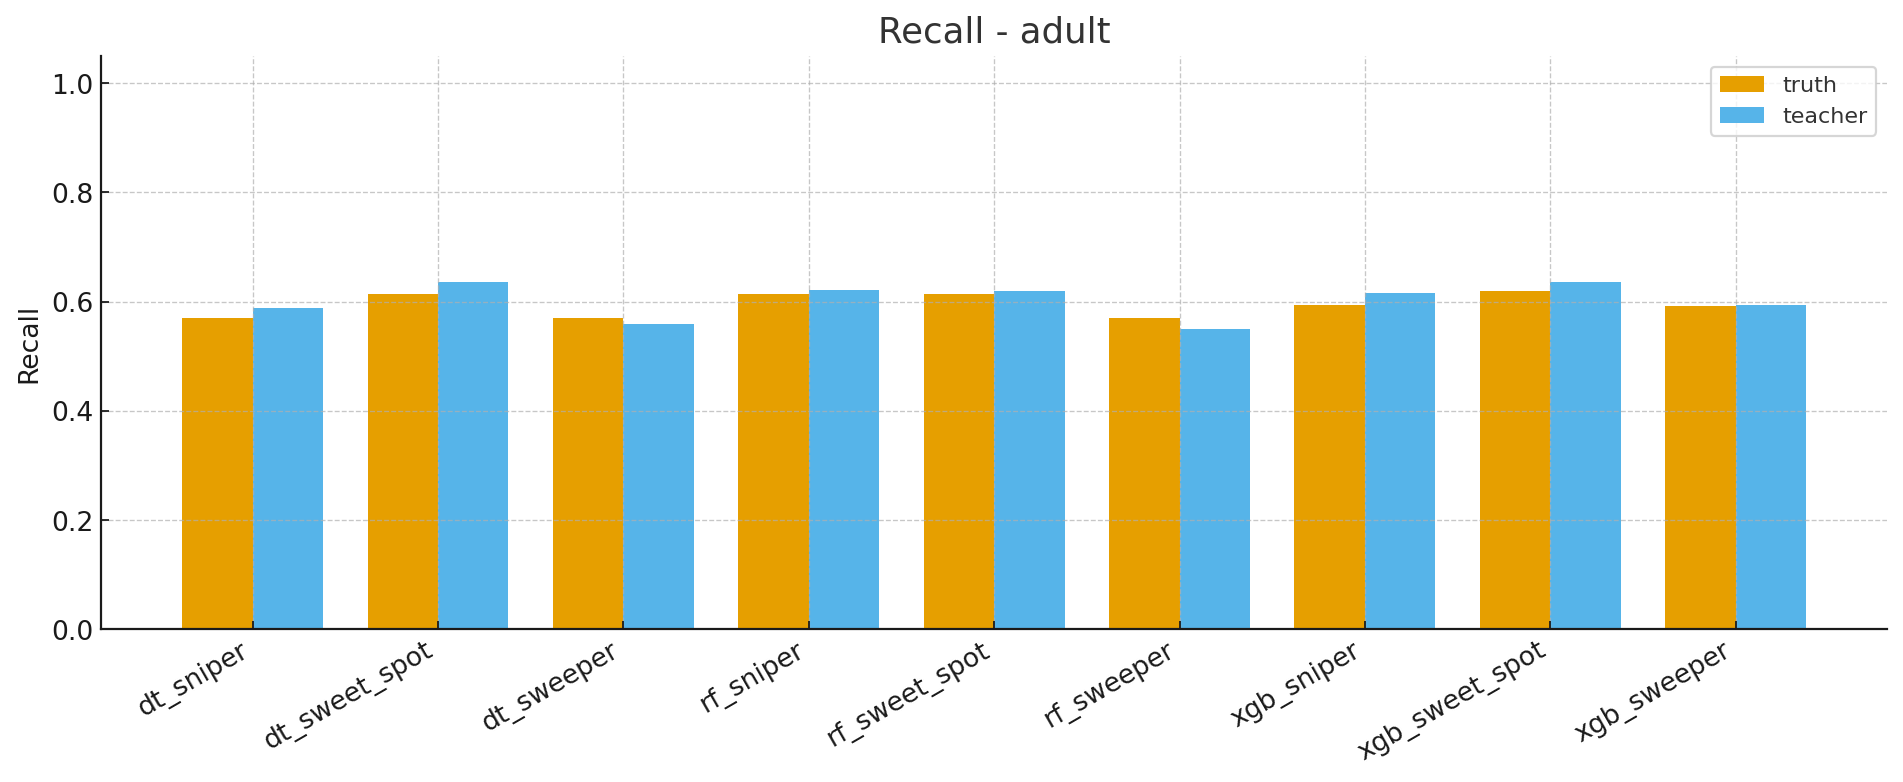
\includegraphics[width=.85\linewidth]{images/charts/recall_simple_adult.png}
  \caption{Recall — \textit{adult}.}
  \label{fig:adult-recall}
\end{figure}

F1 према учитељу је доследно изнад F1 према истини: баланс прецизности и одзива изгледа боље када се мери на учитељским ознакама него на истинитим, што указује на јаку имитацију понашања учитеља уз нешто слабији стварни квалитет. Видети слику \ref{fig:adult-f1}.
\begin{figure}[H]
  \centering
  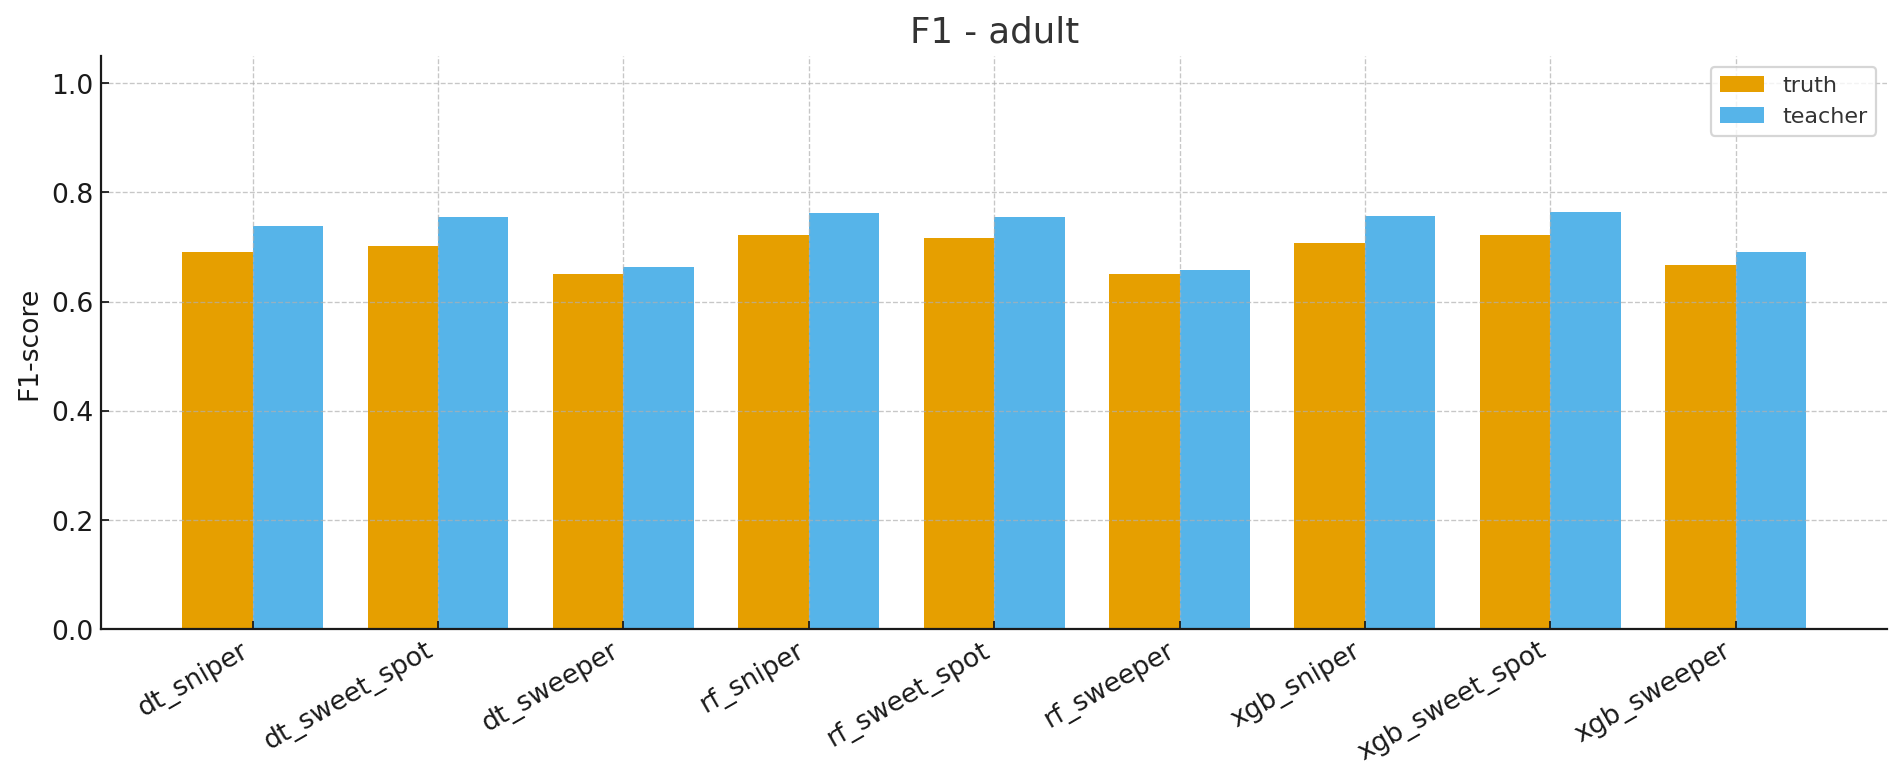
\includegraphics[width=.85\linewidth]{images/charts/f1_simple_adult.png}
  \caption{F1 — \textit{adult}.}
  \label{fig:adult-f1}
\end{figure}

\textit{MCC} према учитељу је у свим поставкама виши: укупни корелациони квалитет предвиђања дестилата боље се слаже са учитељем него са истином, што сугерише да су одлуке дестилата ближе учитељевој граници него стварној дистрибуцији ознака. Видети слику \ref{fig:adult-mcc-tt}.
\begin{figure}[H]
  \centering
  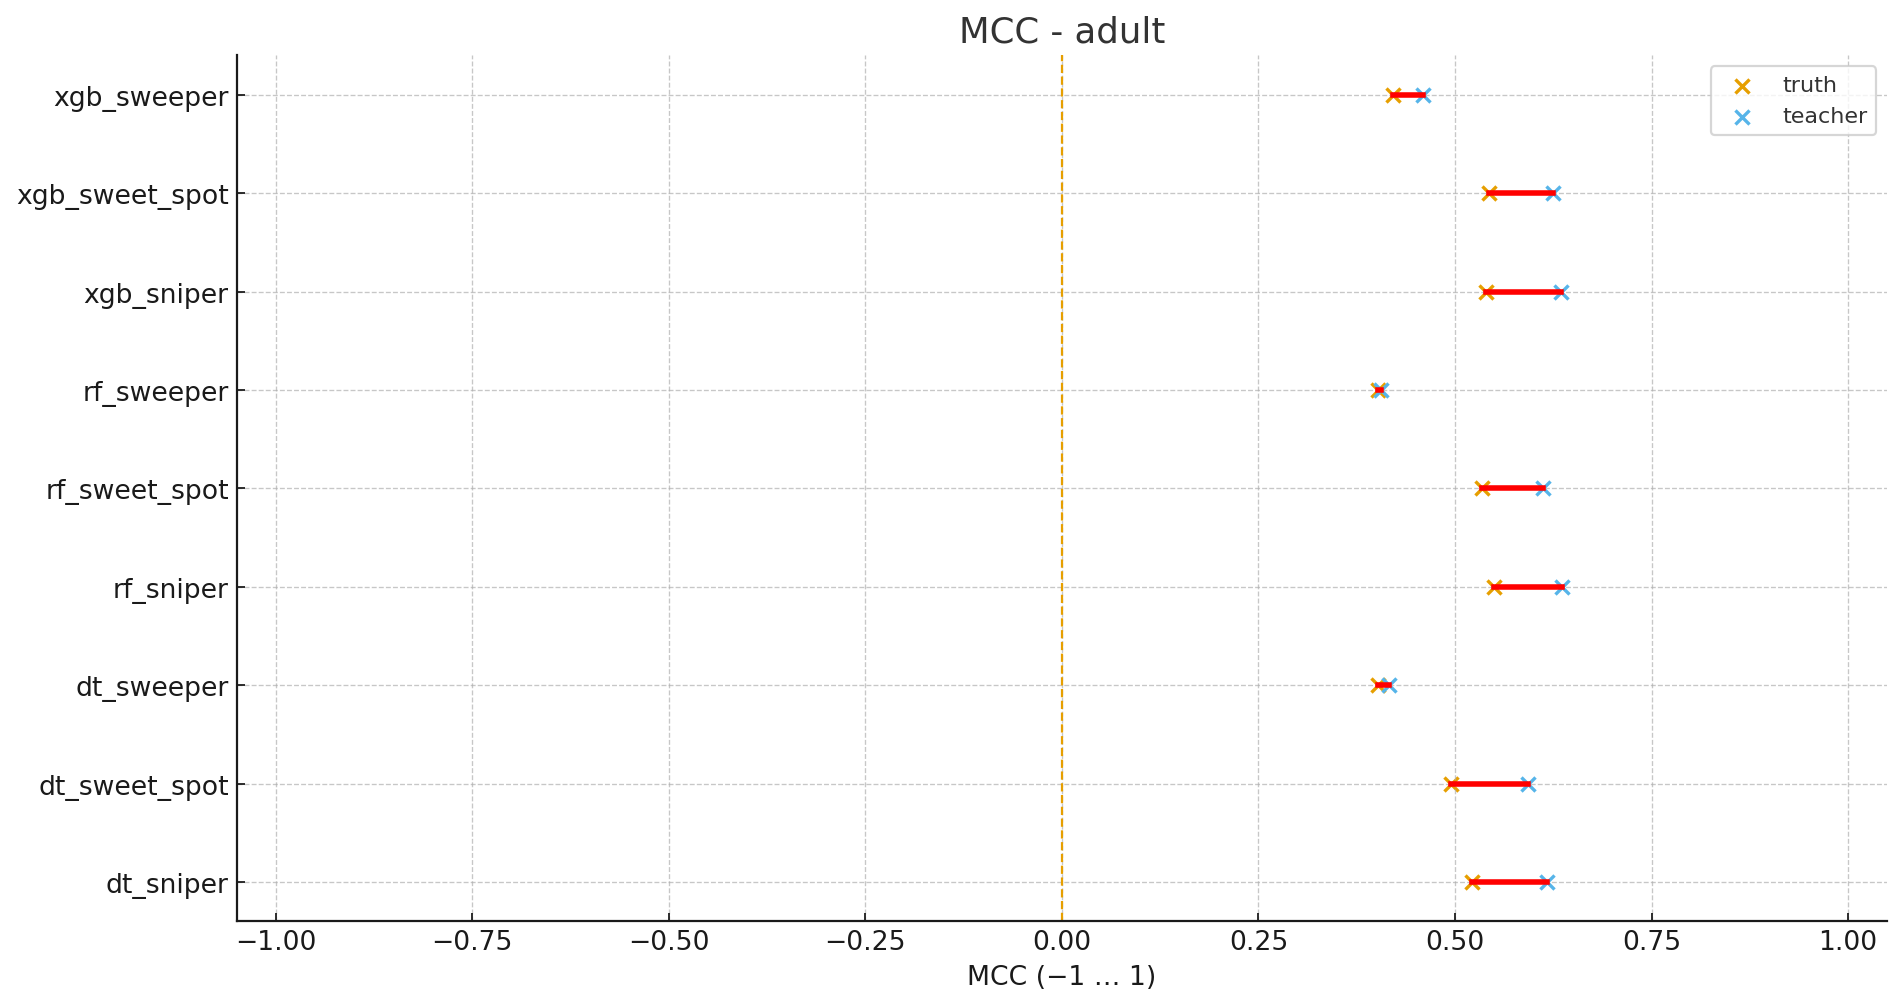
\includegraphics[width=.85\linewidth]{images/charts/mcc_simple_adult.png}
  \caption{\textit{MCC} — \textit{adult}.}
  \label{fig:adult-mcc-tt}
\end{figure}

\subsubsection*{Закључак — \textit{adult}}
Дестилација у Aleph-у открива уобичајени компромис између верности учитељу и стварне тачности према истини: фиделитет је редовно виши од тачности, што указује да дестилати веома успешно имитирају понашање учитеља, али не нужно побољшавају реалну генерализацију. Повећање сложености (више правила и дужа тела) доноси добитке који брзо опадају, \textit{sniper} и \textit{sweet\_spot} дају најбољи однос квалитета и интерпретабилности, док \textit{sweeper} пружа најједноставнија, али и слабија решења (нижи \textit{MCC}). У односу на учитеље, \textit{RF} и \textit{XGB} воде ка дестилатима са стабилнијим метрикама од \textit{DT}-а, што подржава избор ансамбла као учитеља кад је циљ висок фиделитет уз разумну сложеност.

Практично, за \textit{adult} је најисплативије дестилисати \textit{RF}/\textit{XGB} у \textit{sweet\_spot} режиму са умереним ограничењем дужине клаузе (3–4) и строжим \texttt{minacc} (≥0.7–0.8): добијају се компактни скуп(ови) правила који задржавају висок фиделитет и прихватљив реалан квалитет. Имајући у виду да су класе у оригиналу неуједначене (иако су у експерименту избалансиране \textit{undersampling}-ом), за продукциону примену препоручује се (i) провера калибрације и осетљивих метрика, (ii) анализа стабилности правила под различитим шемама дискретизације. Укратко: интерпретабилни дестилати на \textit{adult} могу верно да „преведу“ ансамбл учитеље у логичка правила уз минималан губитак перформанси, под условом да се пажљиво изабере зона компромиса између сложености и квалитета.

\subsection{Контрола компромиса прецизност-одзив}

У литератури је показано да се компромис прецизност-одзив у ИЛП-у може додатно контролисати ансамблирањем клауза по узору на \emph{Gleaner} \cite{Goadrich2006Gleaner}: кандидати се рангирају по одзиву на тренинг/валидацији, оса одзива се дели у $B$ биновa, у сваком бину задржава се до $K$ разноврсних клауза (нпр. по разликама у покривању), а одлука се формира правилом $L$-од-$K$ (пример је позитиван ако га покрива најмање $L$ клауза из датог бина). На тај начин се, без измене саме индукције, генерише читав скуп тачака на PR кривој и максимизује AURPC у окружењима са дисбалансом класа. Приступ је комплементаран „дестилатима“, који померају појединачне тачке кроз подешавања \texttt{evalfn}, \texttt{minacc} и \texttt{noise}. За евалуацију се препоручује угнежђена валидација хиперпараметара $(B,K,L)$ и bootstrap поређење AURPC у односу на базну поставку, уз контролу сложености дедупликацијом клауза, елиминацијом Pareto-доминираних кандидата у (recall, precision) простору и ограничавањем $K$ по бину. Поступак је тривијално паралелизабилан по биновима и/или по скуповима семена. 

% \input{poglavlja/telo/poglavlje3}   % ТОДО направити нова поглавља по узору на poglavlje1 и poglavlje2
\section{Закључак}
Овде врло кратко подсетити на решаван проблем и написати закључке до којих сте дошли. Можете додати и будуће правце рада који нису имплементирани, а могли би допринети побољшању даље студије проблема.         % ТОДО попунити
\newpage

\begin{appendices}

\section{Први додатак}
Додаци су необавезни део рада. Овде се могу убацити сирови подаци на основу којих сте, на пример, нацртали графиконе приказане у телу рада, а којих је исувише да би се приказали у самом телу рада без одвлачења пажње читаоца са шире слике утицаја добијених резултата.

\section{Други додатак}
ТОДО опционо

\end{appendices}
            % ТОДО попунити уколико су вам потребни, додаци могу бити изостављени
\newpage

\bibliographystyle{plain}
\typeout{}
\bibliography{biblist}              % ТОДО попуњавати референцама

\end{document}